%%% The main file. It contains definitions of basic parameters and includes all other parts.

%% Settings for single-side (simplex) printing
% Margins: left 40mm, right 25mm, top and bottom 25mm
% (but beware, LaTeX adds 1in implicitly)
\documentclass[12pt,a4paper]{report}
\setlength\textwidth{145mm}
\setlength\textheight{247mm}
\setlength\oddsidemargin{15mm}
\setlength\evensidemargin{15mm}
\setlength\topmargin{0mm}
\setlength\headsep{0mm}
\setlength\headheight{0mm}
% \openright makes the following text appear on a right-hand page
\let\openright=\clearpage

%% Settings for two-sided (duplex) printing
% \documentclass[12pt,a4paper,twoside,openright]{report}
% \setlength\textwidth{145mm}
% \setlength\textheight{247mm}
% \setlength\oddsidemargin{14.2mm}
% \setlength\evensidemargin{0mm}
% \setlength\topmargin{0mm}
% \setlength\headsep{0mm}
% \setlength\headheight{0mm}
% \let\openright=\cleardoublepage

%% Character encoding: usually latin2, cp1250 or utf8:
\usepackage[utf8]{inputenc}

%% Further useful packages (included in most LaTeX distributions)
\usepackage{amsmath}        % extensions for typesetting of math
\usepackage{amsfonts}       % math fonts
\usepackage{amsthm}         % theorems, definitions, etc.
\usepackage{bbding}         % various symbols (squares, asterisks, scissors, ...)
\usepackage{bm}             % boldface symbols (\bm)
\usepackage{graphicx}       % embedding of pictures
\usepackage{fancyvrb}       % improved verbatim environment
\usepackage[square,numbers]{natbib}         % citation style AUTHOR (YEAR), or AUTHOR [NUMBER]
\usepackage[nottoc]{tocbibind} % makes sure that bibliography and the lists
			    % of figures/tables are included in the table
			    % of contents
\usepackage{dcolumn}        % improved alignment of table columns
\usepackage{booktabs}       % improved horizontal lines in tables
\usepackage{paralist}       % improved enumerate and itemize
\usepackage[usenames]{xcolor}  % typesetting in color
\DeclareGraphicsExtensions{.pdf,.png,.jpg}
\graphicspath{ {../img/} }
\usepackage{listings}
\lstset{columns=flexible}
%%% Basic information on the thesis

% Thesis title in English (exactly as in the formal assignment)
\def\ThesisTitle{Monitoring Tool for Distributed Java Applications}

% Author of the thesis
\def\ThesisAuthor{Bc. Jakub Háva}

% Year when the thesis is submitted
\def\YearSubmitted{2017}

% Name of the department or institute, where the work was officially assigned
% (according to the Organizational Structure of MFF UK in English,
% or a full name of a department outside MFF)
\def\Department{Department of Distributed and Dependable Systems}

% Is it a department (katedra), or an institute (ústav)?
\def\DeptType{Department}

% Thesis supervisor: name, surname and titles
\def\Supervisor{RNDr. Pavel Parízek, Ph.D}

% Supervisor's department (again according to Organizational structure of MFF)
\def\SupervisorsDepartment{Department of Distributed and Dependable Systems}

% Study programme and specialization
\def\StudyProgramme{Computer Science}
\def\StudyBranch{Software Systems}

% An optional dedication: you can thank whomever you wish (your supervisor,
% consultant, a person who lent the software, etc.)
\def\Dedication{%
I would like to thank my thesis supervisor Dr. Pavel Parízek for leading me throughout the whole thesis and willing to help with any concerns I've ever had. I would also like to thank H2O.ai for being able to write this thesis under their coordination, particularly to Dr. Michal Malohlava for providing very useful technical advice.
}

% Abstract (recommended length around 80-200 words; this is not a copy of your thesis assignment!)
\def\Abstract{%
The main goal of this thesis is to create a monitoring platform and library that can be used to monitor distributed Java-based applications. This work is inspired by Google Dapper and shares a concept called "Span" with it. Spans represents a small specific part of the computation and  are used to capture state among multiple communicating hosts. In order to be able to collect spans without recompiling the original application's code, instrumentation techniques are highly used in the thesis. The monitoring tool, which is called Distrace, consists of two parts: the native agent and instrumentation server. Users of this platform are supposed to extend the instrumentation server and specify the points in their application's code where new spans should be created and closed. In order to achieve high performance and affect the running application at least as possible, the instrumentation server is used for instrumenting the code. The tool is aimed to have a small foot-print on the monitored applications, should be easy to deploy and is transparent to target applications from the point of view of the final user.
}

% 3 to 5 keywords (recommended), each enclosed in curly braces
\def\Keywords{%
{monitoring}, {cluster}, {instrumentation}, {distributed systems}, {performance}
}

%% The hyperref package for clickable links in PDF and also for storing
%% metadata to PDF (including the table of contents).

\usepackage[pdftex,unicode]{hyperref}   % Must follow all other packages
\hypersetup{breaklinks=true}
\hypersetup{pdftitle={\ThesisTitle}}
\hypersetup{pdfauthor={\ThesisAuthor}}
\hypersetup{pdfkeywords=\Keywords}
\hypersetup{urlcolor=blue}
% Definitions of macros (see description inside)
%%% This file contains definitions of various useful macros and environments %%%
%%% Please add more macros here instead of cluttering other files with them. %%%

%%% Minor tweaks of style

% These macros employ a little dirty trick to convince LaTeX to typeset
% chapter headings sanely, without lots of empty space above them.
% Feel free to ignore.
\makeatletter
\def\@makechapterhead#1{
  {\parindent \z@ \raggedright \normalfont
   \Huge\bfseries \thechapter. #1
   \par\nobreak
   \vskip 20\p@
}}
\def\@makeschapterhead#1{
  {\parindent \z@ \raggedright \normalfont
   \Huge\bfseries #1
   \par\nobreak
   \vskip 20\p@
}}
\makeatother

% This macro defines a chapter, which is not numbered, but is included
% in the table of contents.
\def\chapwithtoc#1{
\chapter*{#1}
\addcontentsline{toc}{chapter}{#1}
}

% Draw black "slugs" whenever a line overflows, so that we can spot it easily.
\overfullrule=1mm

%%% Macros for definitions, theorems, claims, examples, ... (requires amsthm package)

\theoremstyle{plain}
\newtheorem{thm}{Theorem}
\newtheorem{lemma}[thm]{Lemma}
\newtheorem{claim}[thm]{Claim}

\theoremstyle{plain}
\newtheorem{defn}{Definition}

\theoremstyle{remark}
\newtheorem*{cor}{Corollary}
\newtheorem*{rem}{Remark}
\newtheorem*{example}{Example}

%%% An environment for proofs

%%% FIXME %%% \newenvironment{proof}{
%%% FIXME %%%   \par\medskip\noindent
%%% FIXME %%%   \textit{Proof}.
%%% FIXME %%% }{
%%% FIXME %%% \newline
%%% FIXME %%% \rightline{$\square$}  % or \SquareCastShadowBottomRight from bbding package
%%% FIXME %%% }

%%% An environment for typesetting of program code and input/output
%%% of programs. (Requires the fancyvrb package -- fancy verbatim.)

\DefineVerbatimEnvironment{code}{Verbatim}{fontsize=\small, frame=single}

%%% The field of all real and natural numbers
\newcommand{\R}{\mathbb{R}}
\newcommand{\N}{\mathbb{N}}

%%% Useful operators for statistics and probability
\DeclareMathOperator{\pr}{\textsf{P}}
\DeclareMathOperator{\E}{\textsf{E}\,}
\DeclareMathOperator{\var}{\textrm{var}}
\DeclareMathOperator{\sd}{\textrm{sd}}

%%% Transposition of a vector/matrix
\newcommand{\T}[1]{#1^\top}

%%% Various math goodies
\newcommand{\goto}{\rightarrow}
\newcommand{\gotop}{\stackrel{P}{\longrightarrow}}
\newcommand{\maon}[1]{o(n^{#1})}
\newcommand{\abs}[1]{\left|{#1}\right|}
\newcommand{\dint}{\int_0^\tau\!\!\int_0^\tau}
\newcommand{\isqr}[1]{\frac{1}{\sqrt{#1}}}

%%% Various table goodies
\newcommand{\pulrad}[1]{\raisebox{1.5ex}[0pt]{#1}}
\newcommand{\mc}[1]{\multicolumn{1}{c}{#1}}

% Title page and various mandatory informational pages
\begin{document}
%%% Title page of the thesis and other mandatory pages

%%% Title page of the thesis

\pagestyle{empty}
\hypersetup{pageanchor=false}
\begin{center}

\centerline{\mbox{
\includegraphics[width=166mm]{../img/logo-en.pdf}}}

\vspace{-8mm}
\vfill

{\bf\Large MASTER THESIS}

\vfill

{\LARGE\ThesisAuthor}

\vspace{15mm}

{\LARGE\bfseries\ThesisTitle}

\vfill

\Department

\vfill

\begin{tabular}{rl}

Supervisor of the master thesis: & \Supervisor \\
\noalign{\vspace{2mm}}
Study programme: & \StudyProgramme \\
\noalign{\vspace{2mm}}
Study branch: & \StudyBranch \\
\end{tabular}

\vfill

% Zde doplňte rok
Prague \YearSubmitted

\end{center}

\newpage

%%% Here should be a bound sheet included -- a signed copy of the "master
%%% thesis assignment". This assignment is NOT a part of the electronic
%%% version of the thesis. DO NOT SCAN.

%%% A page with a solemn declaration to the master thesis

\openright
\hypersetup{pageanchor=true}
\pagestyle{plain}
\pagenumbering{roman}
\vglue 0pt plus 1fill

\noindent
I declare that I carried out this master thesis independently, and only with the cited
sources, literature and other professional sources.

\medskip\noindent
I understand that my work relates to the rights and obligations under the Act No.~121/2000 Sb.,
the Copyright Act, as amended, in particular the fact that the Charles
University has the right to conclude a license agreement on the use of this
work as a school work pursuant to Section 60 subsection 1 of the Copyright Act.

\vspace{10mm}

\hbox{\hbox to 0.5\hsize{%
In ........ date ............	% FIXME!
\hss}\hbox to 0.5\hsize{%
signature of the author
\hss}}

\vspace{20mm}
\newpage

%%% Mandatory information page of the thesis

\openright

\vbox to 0.5\vsize{
\setlength\parindent{0mm}
\setlength\parskip{5mm}

Title:
\ThesisTitle

Author:
\ThesisAuthor

\DeptType:
\Department

Supervisor:
\Supervisor, \SupervisorsDepartment

Abstract:
\Abstract

Keywords:
\Keywords

\vss}

\newpage

%%% Dedication

\openright

\noindent
\Dedication

\newpage

\openright
\pagestyle{plain}
\pagenumbering{arabic}
\setcounter{page}{1}


%%% A page with automatically generated table of contents of the master thesis
\setcounter{tocdepth}{1}
\tableofcontents

%%% Each chapter is kept in a separate file
%%\chapter*{Introduction}
\addcontentsline{toc}{chapter}{Introduction}


\chapter{Introduction}
\section{Project Goals}


\chapter{Background}
\label{chap:background}
This chapter covers technologies relevant to the thesis. It starts with an overview of similar monitoring tools for cluster-based applications and follows by short overview of tools used for debugging of large scale applications. Different approaches to applications profiling are described in the following part. 

In the next several sections the technologies considered to be used in Distrace or used in thesis are introduced. The sections cover libraries for bytecode manipulation, communication, logging and also cover important relevant parts of Java libraries such as JNI and JVMTI. Docker is briefly described at the end of this chapter as it is used as the main distribution package of the whole platform.

\section{Cluster Monitoring Tools}
The most significant and relevant platforms on which this thesis is inspired are Google Dapper, Zipkin and HTrace. All three tools serve the same core purpose, which is to monitor large-scale Java-based distributed applications. Zipkin and HTrace are developed according to Google Dapper design and therefore these three platforms share a few similar concepts. The basic concept shared between the platforms is a concept called \textit{Span}. Spans are structures used to collect the shared state between the application nodes and usually encapsulate a few calls between the neighboring nodes with well-defined start and end of the communication. They are formed in hierarchical structures called trace trees, in which the user can see how distributed calls related on each other. Spans are explained in more details later in the following sections. 

The following three sections describe the basics of each of the mentioned platforms. Since Zipkin, HTrace and Google Dapper share some basic concepts, only those parts of each platform that are relevant and interesting to the thesis are described.
\subsection{Google Dapper}
\label{dapper}
Google Dapper is a proprietary software used at Google. It is mainly used as a tool for monitoring large distributed systems and helps with debugging and reasoning about applications performance running on multiple host at the same time. Different parts of the monitored system does not have to be written in the same programming language. Google Dapper has three main pillars on which is built:
\begin{itemize}
	\item \textbf{Low overhead} \newline
	Google Dapper should share the same life-cycle as the monitored application itself to capture also the intermittent events and thus low overhead is one of the main design goals of the tool.
	\item \textbf{Application level transparency} \newline
	The developers and users of the application should not need to know about the monitoring tool and are not supposed to change the way how they interact with the system when the monitoring tool is running. It can be assumed from the paper that achieving application level transparency at Google was easier than it could be in more diverse environments since all the code produced at the Google use the same libraries and share similar control flow practices.
	\item \textbf{Scalability} \newline
	Such a system should perform well on data of significantly large scale.
\end{itemize}	
Google Dapper collects the information from distributed applications as distributed traces. The origin of the distributed trace is the communication or task initiator and the trace spans across the nodes in the cluster also participating in the computation or communication.
	
There were two proposed approaches for obtaining the distributed traces when Google Dapper was developed: black-box and annotation-based monitoring approaches. The black-box approach assumes no additional knowledge about the application whereas the annotation-based approach can make use of additional information via annotations. Google Dapper is mainly using black-box monitoring schema since most of the control flow and RPC (Remote Procedure Call) subsystems are shared among Google, however support for custom annotations is provided via additional libraries build on top of the core system. This gives the developer of an application possibility to attach some additional information to spans, which are very application-specific.
	
In google Dapper, distributed traces are represented as so called trace trees, where tree nodes are basic units of work referred to as spans. Spans are related to other spans via dependency edges. These edges represents relationship between parent span and children of this span. Usually the edges represent a set of related RPC calls or similar kind of communication. Each span can be uniquely identified using its id. In order to reconstruct the whole trace tree, the monitoring tool needs to be able to identify the span where the computation started. Spans without parent id are called root spans and serve exactly this purpose. Spans can also contain information from multiple hosts, usually from direct neighborhood of the span. Structure of a span in Google Dapper platform is described in the Figure \ref{fig:dapper_span}. The figure shows a single span encapsulating the client-server communication. It can be seen that events from both nodes are recorded within a single span.
\begin{figure}
	\centering
		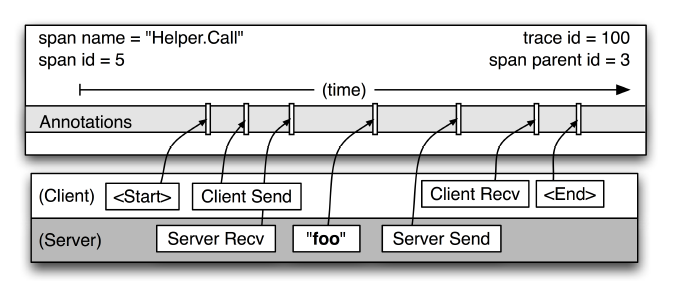
\includegraphics[scale=0.7]{dapper_span.png}
	\caption{Example of of a span in Google Dapper. Picture taken from the Google Dapper paper}
	\label{fig:dapper_span}
\end{figure}

Google Dapper is able to follow distributed control paths thanks to instrumentation of a few common shared libraries among Google developers. This instrumentation is not visible to the final users of the system and therefore Dapper has high-level of application transparency. Instrumentation in Dapper is achieved by tracing three main instrumentation points. 
\begin{itemize}
	\item Dapper attaches a so called trace context as thread-local variable to the current thread when the thread handles any kind of traced control path. Trace context is a small data structure containing mainly reference to a current and parent span via their ids.
	
	\item In distributed systems the communication is often done via callbacks. Callback is a method which is usually executed when some execution in different part of the application has finished. Dapper instruments the callback mechanism so when computation is deferred, traced callbacks still carry around the trace context of the creator and therefore also parent and current span ids.
	
	\item Most of the communication in Google is using single RPC framework with language bindings to different languages. This library is instrumented as well to achieve the desired application-level transparency.
\end{itemize}

Sampling of the captured data has also a positive effect on the low-level overhead of the whole application. As mentioned in the paper, the volume of data processed at Google is significant so only samples are taken at a time.

\subsection{Zipkin}
\label{zipkin}
Zipkin is an open-source distributed tracing system. It is based on Google Dapper technical paper and manages both the collection and lookup of the captured data. Zipkin uses instrumentation and annotations for capturing the data. Some
information are recorded automatically, for example time when a span was created, whereas some information are optional. Zipkin has also support for custom application-specific annotations.

Zipkin architecture can bee seen on Figure \ref{fig:zipkin_architecture}.
\begin{figure}
	\centering
	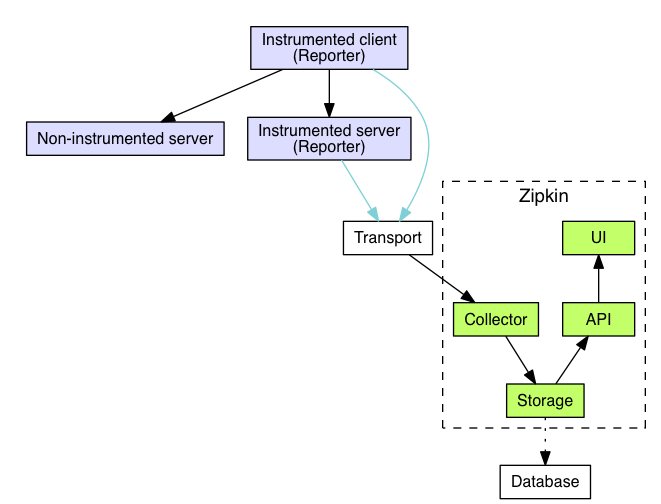
\includegraphics[scale=0.6]{zipkin_architecture.png}
	\caption{Zipkin architecture - http://zipkin.io/pages/architecture.html}
	\label{fig:zipkin_architecture}
\end{figure}
The instrumented application is responsible for creating valid traces. For that reason, Zipkin has set of pre-instrumented libraries ready to be used in order to work well with the whole Zipkin infrastructure. Spans are stored asynchronously in Zipkin to ensure lower overhead. Once a span is created by the application, it is sent to Zipkin collector. In General, Zipkin consists of four components:
\begin{itemize}
	\item \textbf{Zipkin Collector} \newline
	The collector is usually a daemon thread or process which stores, validates and indexes the data for future lookups.
	\item\textbf{Storage} \newline
	Data in Zipkin can be stored in multiple ways which makes this is a pluggable component. For example, data can be stored in Cassandra, MySQL or can be send to Zipkin user interface right away without any intermediate storage. The last option is good for handling a small amount of data since the user interface is not supposed to handle storing data of big size.
	\item \textbf{Zipkin Query Service} \newline
	This component acts as a query daemon allowing the user to query various information about spans using simple JSON API.
	\item \textbf{Web UI} \newline
	A basic, but very useful user interface. It allows the user to see whole trace trees and all spans with dependencies between them. The user interface accepts the spans in JSON format.
\end{itemize}
The Zipkin Web UI is used as a front-end  for the monitoring tool developed in the scope of this thesis. More information on how the user interface is used in Distrace tool is described in more details in section 4.6 \hyperref[sec:zipkin_ui]{Zipkin UI} of \hyperref[chap:design]{Design} chapter.
 \section{HTrace}
 \label{htrace}
 HTrace https://github.com/cloudera/htrace is a tracing framework created by Cloudera used for monitoring distributed systems written in Java. It is based on Google Dapper as well and shares the same concepts such as spans and trace trees. In order to allow tracing of the application, the users need to manually attach a span identifiers to desired RPC calls (Remote Procedure Calls). These identifiers are then used to create relationships between spans collected on different nodes. HTrace stores the span and trace information in thread-local storage and the user is responsible for making sure this state is transferred to a new thread or node. Htrace has also support for custom spans annotations and thus allows the user to collect application specific information as part of the spans. 
 
 The disadvantage of this tool is the need for instrumenting the monitored application in order to allow the tracing and spans collection.
\section{Tools for Large-Scale Debugging}
Standard techniques and tools can be used for debugging distributed applications, however the main purpose of these tool is to debug single node applications and therefore when applying them on nodes in the distributed application the information about dependencies between different nodes in the cluster is not available. Many tools for large-scale debugging exist, but this section just points out basic ideas behind two different approaches - discovering scaling bugs and behavior based debugging. 

\subsection{Discovering Scaling Bugs}
The scalability is one of the most important aspects of distributed systems. It is desirable to know how the platform scales when it process significantly large data and what is the expected scalability trend. It can happen that the platform can run significantly slower on big data than expected after testing on smaller data. This issue is usually called a scaling bug. Tools which can be used to help discovering scaling bugs are for example Krishna and WuKong. Both of the mention tools are based on the same idea. They build a scaling trend based on data batches of smaller size and the observed scaling trend acts as a boundary. The scaling bug becomes observable when the scaling trend is violated. The first tool, Krishna, is not able to distinguish which part of the program violated the scaling trend. This is however possible in the second tool, WuKong. In comparison to Krishna, Wukong does not build one scaling trend of the whole application, but creates more smaller models, each per some control flow structure in desired programming language. All these smaller models represent together the whole scaling trend. When the application observes the scaling bug, WuKong is able to locate the developer in the place in the code where the trend is probably violated.

\subsection{Behavior-based Analysis}
The second category of tools used for debugging large scale applications are based on behavior analysis. The basic idea behind these tools is creation of classes of equivalence from different runs and processes of the application. Using this approach, the amount of data used for further inspection is reduced down. These tools are especially helpful when discovering anomalies between different observed application runs. For example, STAT - Stack Trace Analysis Tool, is a lightweight and scalable debugging tool used for identifying errors on massive high performance computing platforms. It gathers stack traces from all parallel executions, merges together stack traces from different processes that have the same calling sequence and based on that creates equivalence classes which make it easier for debugging highly parallel applications. 

The other tool used as an example in this category is AutomaDed. This tool creates several models from an application run and can compare them using clustering algorithm with (dis)-similarity metric to discover anomalous behavior. It can also point to specific code region which may be causing the anomaly.

\section{Profiling Tools}
Profiling is a form of dynamic code analysis. It may be used for example for determining how long each part of the system takes compared to the time of whole application run or for example to determine which part of the application uses the most memory. Profiling tools can be divided in two categories:
\begin{itemize}
	\item \textbf{Sampling Profilers} \newline
Sampling profilers take statistical samples of an application at well-defined points such as method invocations. The points where the application should take samples have to be inserted at the compilation time by the compiler. Sampling profilers usually have less overhead compared to instrumentation profilers. These profiles are good to collect for example time how long a method run, caller of the method or for example the complete stacktrace. However they are not able to collect any application specific information.
	\item \textbf{Instrumentation Profilers} \newline
This can be solved by instrumentation profilers. These profilers are based on the instrumentation of the application's source code. They record the same kind of information as the sampling profilers and usually give the developer the ability to specify extra points in the code where the application specific data ar recorded. Compared to sampling profilers, instrumentation profilers usually have slightly worse performance.
\end{itemize}

However, profilers can be also looked at from different point of view and categorized based on the level on which they operate and are able to record the information.
\begin{itemize}
	\item \textbf{System Profilers} \newline
	System profilers operate on operating system level. They can show system code paths, but are not able to capture method calls done for example in Java application.
	\item \textbf{Application Specific Profilers} \newline
	Generally, application specific profilers are able to collect method calls within the application. For example, JVM profilers can show Java stack traces but are not able to show the further call sequence on the operating system level.

\end{itemize}
The ideal solution for monitoring purposes of Java applications would be to have information from both kind of profilers, however combining outputs of these profiler types is not straightforward. The profilers which are able to collect traces from both system and JVM profilers are usually called mixed-mode profilers. JDK8u60 comes with the solution in a form of extra JVM argument \textit{-XX:+PreserveFramePointer} \cite{MixedModeProfilers}.  Operating system is usually using this field to point to the most recent call on the stack frame and system profilers make uses of this field. In case of Java, compilers and virtual machines don't need to use this field since they are able to calculate the offset of the latest stack frame from the stack pointer. This leaves this register available for various kind of JVM optimizations. The \textit{-XX:+PreserveFramePointer}  option ensures that JVM abides the frame pointer register and will not use it as a general purpose register. Therefore, both system and JVM stack frames can appear in single call hierarchy. Using the JVM mixed-mode profilers we are able to collect stack traced leading to:
\begin{itemize}
	\item \textbf{Page Faults} - these traces are useful to show what JVM code triggered main memory to grow.
	\item \textbf{Context Switches} - these traces are used to determine code paths which often lead to CPU switches.
	\item\textbf{Disk I/O Requests} - these traces show code paths leading to IO operations such as blocking disk seek operation.
	\item \textbf{TCP Events} - these traces show code paths going from high-level Java code to low-level system methods such as \texttt{connect} or\texttt{ accept}. They can be used to reason about performance and good design of network communication in much more better detail.
	\item \textbf{CPU Cache Misses} - these traces show code paths leading to cache misses. This information can be used to optimize the Java code to make better use of the existing cache hierarchy.
\end{itemize}

All the information bellow can be described on a special chart called Flame charts.
\subsubsection{Flame Graphs}
Flame Graphs are special graphs introduced developer Brendan Gregg. Flame graphs are visualization for sampled stack traces, which allows the hot paths in the code to be identified quickly. The output of sampling or instrumentation profiler can be significantly big and therefore visualizing can help to reason about performance in more comfortable way. 

\begin{figure}
	\centering
	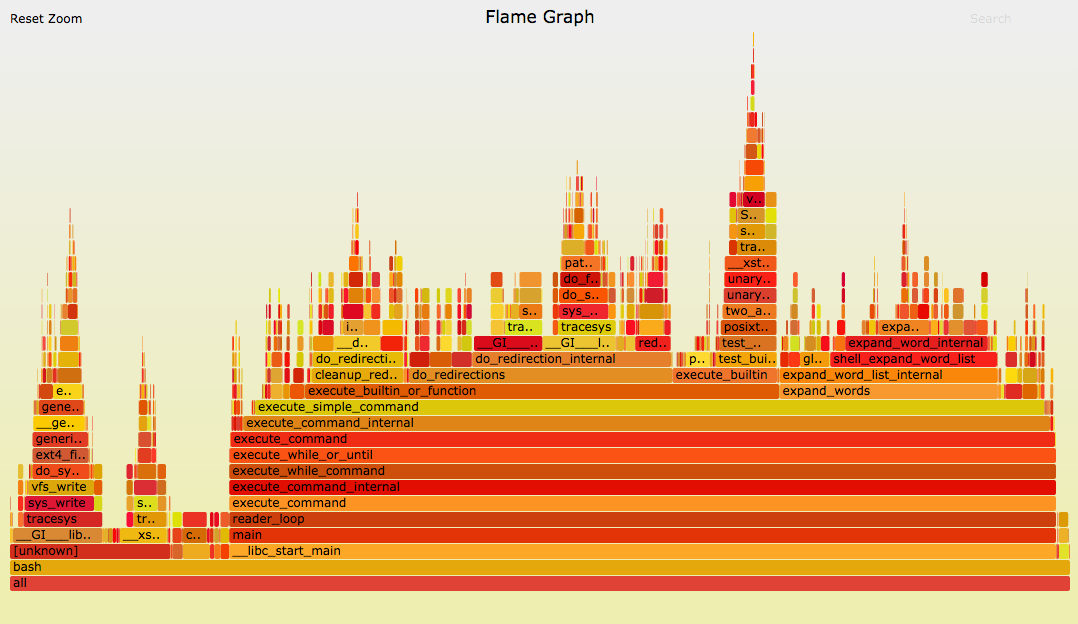
\includegraphics[scale=0.35]{flame_chart.png}
	\caption{Flame Graph example}
	\label{fig:flame_chart}
\end{figure}
Flame graph is a graph where:
\begin{itemize}
	\item Each box represents a function call in the stack.
	\item The \textbf{y-axis} shows stack frame depth. The top function is the function which was at the moment of capturing this flame chart on the CPU. All functions underneath of it are its ancestors.
	\item The \textbf{x-axis} shows the population of traces. It doesn't represent passage of time. The function calls are usually sorted alphabetically.
	\item The width of each box represents the time how long the function was on CPU.
	\item The colors are not significant, they are just used to visually separate different function calls.
\end{itemize}

Flame charts can be created in a few simple steps, but it depends on the type of profiler the user wants to use. 
\begin{enumerate}
	\item Capture stack traces. For this step the profiler of custom choice may be used.
	\item Fold stacks. The stacks need to be prepared so Flame graphs can be created out of them. Scripts for most of the major profilers exist and may be used to prepare the folded stack trace.
	\item Generate the flame graph itself again using the helper script.
\end{enumerate}

The purpose of this really short section is just to introduce the idea of Flame charts because it's one of the future plans to add support for flame charts into to monitored tools developed by this thesis. For more information about the flame charts please visit the Brendan Gregg's blog.
\section{Byte Code Manipulation Libraries}
The thesis highly depends on the Java bytecode instrumentation and this section gives overview of four bytecode manipulation libraries considered to be used at the thesis:  Javassist, Byte Buddy, CGlib and. Since it's a core feature of the whole platform and affects both the performance and the usability of the whole platform, the library was thoroughly reviewed before selected. Byte Buddy library was selected and is therefore described in more detail. However the reasons for its selection can be found in the following \hyperref[analysis]{Analysis} section.

\subsection{ASM}
\label{asm}
ASM is a low-level high-performance Java bytecode manipulation framework. It can be used to dynamically create new classes or redefined already existing classes. It works on the bytecode level so the user of this library is expected to understand the JVM bytecode in detail. ASM operates on event-driven model as it makes use of Visitor design pattern to walk through complex bytecode structures. ASM defines some default visitors such as \textit{FieldVisitor}, \textit{MethodVisitor} or \textit{ClassVisitor}. The ASM project can be a great fit for project requiring a full control over the bytecode creation or inspection since it's low-level nature.
\subsection{Javassist}
\label{javassist}
Javassist is well-known bytecode manipulation library built on top of ASM. It allows the Java programs to define new classes at run-time and also to modify class files prior the JVM loads them. It works on higher level of abstraction compared to ASM so the user of this library is not required to work with the low-level bytecode. The advantage of Javassist is that the injected code does not depend on the Javassist library at all. The code to be injected to the existing bytecode is expressed as Java Strings. The disadvantage of this approach is that the the code to be injected is not subject to code inspection in most of the current IDEs. The strings representing the code are compiled at run-time by special Javassist compiler. This run-time compilation works well for most of the common programming structures but for example auto-boxing and generics are not supported by the compiler. Also it is important to mention that Javassist does not have support for the code injection itself. Therefore, it can be used for specifying the code which alters the original code but external tool needs to be used to inject the code itself.
\subsection{CGLib}
\label{cglib}
CGLib as another byte-code manupulation library built on top of ASM. The main concepts are build around `Enhancer` class which is used to create proxies by dynamically extending classes at run-time. The proxified class is then used to intercept method calls and the result of previous methods or fields as we define. However CGLib lacks comprehensive documentation making harder to even understand the basics.

\subsection{Byte Buddy}
\label{sec:byte_buddy}
Byte Buddy is fairly new, light-weight and high-level bytecode manipulation library. The library depends only on visitor API of the ASM library which does not further have any other dependencies. It does not require from the user to understand format of java bytecode but despite this, it gives the users full flexibility to redefine the bytecode according to their specific needs. Also, classes created or instrumented by Byte Buddy does not depend on the Byte Buddy framework. Despite it's high-level approach, it still offers great performance and is used at frameworks such as Mockito or Hibernate. Byte Buddy can be used for both code generation and transformation of existing code.

\subsubsection{Code Generation}
Code generation is done by specifying from which class a new class should be sub-classing. In the most generic case, class can be created based on the \texttt{Object} class. The newly created class can introduce new methods or intercept methods from it's super class. In order to intercept existing methods (change their behavior and return value), the method to be intercepted has to be identified using so-called \texttt{ElementMatchers}. These matchers allow the developer to identify methods using for example their names, number of arguments, return types or associated annotations. The whole list of matchers and also examples how code can be generated is greatly described in the documentation of the Byte Buddy library.

The power behind Byte Buddy is also that it can be used to redefine classes at run-time. This is achieved by several concepts, mainly via Transformers, Interceptors and Advice API.
\subsubsection{Code Transformation}
In order to tell Byte Buddy what method or field to intercept, the place in code which triggers the interception has to be identified. First,  a class containing the desired method for instrumentation needs to be located. It can be done by simply specifying the class name or using more complex structures. For example, the element marchers may be used to only consider all classes A extending class B whilst implementing interface C at the same type. 

The next step is to define the \texttt{Transformer} class itself. Transformers are used to identify methods in the class which should be instrumented and they also specify the class responsible for the instrumentation itself. This class may be either Interceptor or Advice and their description is given in more detail in the following section. 

The methods to be instrumented can specified in the transformer using the element matchers. In more detail, \texttt{Transformer} interface has a method \texttt{ transform} which has \texttt{DynamicType.Builder} as it's argument. This builder is used to create a single transformer wrapping all the transformers for all classes in the code so the result of this builder can be thought of as a dispatcher of the instrumentation for complete application.

There are two ways how to instrument a class in Byte Buddy. Either via Interceptors or via Advice API.
\subsubsection{Interceptors}
Interceptor is a class defining the new or changed desired behavior for the method to be instrumented. 
The demonstration how Byte Buddy uses interceptors is shown on a small example. Let's assume the class \texttt{Foo} is the original unchanged class:
\begin{lstlisting}[language=Java]
class Foo {
	String bar() {
		return "bar"; 
	}
}
\end{lstlisting}
	
Le'ts also assume that the Interceptor is of type \texttt{Qux}. The interception of the class \texttt{Foo} using the defined interceptor looks like this in schematic code:

\begin{lstlisting}[language=Java]
class Foo {
	// Requires your interceptor class to be known
	static Qux $interceptor;
	String bar() {
		return $interceptor.intercept(); 
	}
	static {
		// Requires knowing the framework
		$interceptor = ByteBuddyFramework.defineField(Foo.class);
	}
}
\end{lstlisting}
		
It can therefore be seen that in case of interceptors, Byte Buddy does not inline the bytecode to the \texttt{Foo} class but requires the interceptor class to be available on the machine where the instrumentation takes place. Also the interceptor field needs to be initialized, which is in this case done in the static initializer. The initialization of interceptors is done using special helper class called \texttt{LoadedTypeInitializer}.

There are multiple ways how this behavior can be changed:
\begin{enumerate}
\item In Byte Buddy, the initialization strategy can be modified accordingly to the specific needs. No-op strategy can be used and \texttt{LoadedTypeInitializer} can be read right before the class is about to be instrumented.  The initialization of the interceptor field can be handled manually later using observed initializer or we can even serialize the initializer together with the \texttt{Qux} \texttt{Interceptor} class, send them to different JVM where the instrumentation should take place and manually initialize the the interceptor field.
\item Instead of referring to \texttt{Qux} as a instance, it can delegated to as instance of \texttt{Qux} class. In this case the interception is performed via static methods and no intializers are required to be available, however the interceptor class still needs to be known at run-time.
\item Instead of using interceptors, advice API which in-lines the code to the class itself may be used.
\end{enumerate}
\subsubsection{Advice API}
Advices are another approach how code can be instrumented in Byte Buddy. This approach is more limited compared to the interceptors, but in cases where it's possible to use it, the code is in-lined into the original class's bytecode and therefore no other dependencies are required. It is also stated in Byte Buddy documentation that performance of Advice API is better compared to the performance if interceptors.
However, the instrumentation using Advice API is only allowed before or after the matched method. This is achieved using the \texttt{Advice.onMethodEnter} and \texttt{Advice.onMethodExit} annotations.

\section{Communication Middleware}
This thesis consist of several parts written in different languages which need be able to communicate. In order to achieve communication in such an environment, following libraries have been inspected.
\subsection{Raw Sockets}
\label{raw_sockets}
It this case raw sockets is not a library but it is referred to as using raw sockets on their low-level API. Using raw sockets has several pros and cos. It give the user full flexibility and the highest possible performance since there isn't any additional layer between the application data and the socket itself. However, integrating different platforms and different languages can be time consuming. Several frameworks have already been created to hide the implementation details of specific platforms so the user does not need to know about the language or underlying platform.
\subsection{ZeroMQ}
\label{zeromq}
ZeroMq is a communication library built on top of raw sockets. The core of the library is written in C++ however binding into different languages exist. The library is able transport messages inside a single process, between different processes on the same node or transfer messages over the network using TCP or also using multicast. The library also allows the user to create typologies using one of the many supported communication patterns. For example,  publisher-subscriber or request-reply patterns are supported. The library has several benefits compared to raw sockets:
\begin{itemize}
	\item Hiding the differences between underlying operating systems.
	\item Message framing - delivering whole messages instead of stream of bytes.
	\item Automatic message queuing. The internals take care of ensuring the messages are sent and received in correct order. The user can send the messages without knowing whether there are other messages in the queue or not.
	\item Language mappings to different languages.
	\item Ability to create different topologies. Example of a topology can be that one socket can be connected to multiple endpoints.
	\item Automatic TCP re-connection
	\item Zero-copy
\end{itemize}
\subsubsection{Zero-copy in ZeroMQ}
The library tries to apply concept called zero-copy whenever possible. When high-performance is expected from a system or network, copying of data is usually considered harmful and should be minimized as possible. The technique of avoiding copies of data is known as zero-copy.

Example of data copying can be transferring data from memory to network interface or from user application to underlying kernel.  It  can be seen that zero-copy can't be implemented at all layers. For instance,  without copying the data from the kernel to network interface, no data could be actually exchanged. However, ZeroMQ can achieve zero-copy at least on the application message level so the users can create ZeroMQ messages from their data without any copying which is a big performance benefit.
\subsection{NanoMsg}
\label{nanomsg}
NanoMsg [http://nanomsg.org/documentation-zeromq.html] is a socket library shadowing the differences between the underlying operation systems. It offers several communication patterns, is implemented on C and does not have any other dependencies. Generally, it offers very similar features to ZeroMQ since it's heavily based on it.

Unlike ZeroMQ, Nanomsg matches the full POSIX compliance. The author of the library states, that since it's implemented in C, the number of memory allocations is drastically reduced compared to c++, where, for example, C++ STL containers are used  Also compared to ZeroMQ, objects are not tightly bound to particular threads. This gives the user flexibility to create their custom threading models without significant limitations. NanoMsg also implements zero-copy technique at additional layers which again leads to performance benefits compared to ZeroMQ.

As in ZeroMQ, NanoMsq supports the following transport mechanisms:
\begin{itemize}
	\item \textbf{INPROC} \newline
	Inter process communication is used for transporting messages withing a single process, for example between different threads. In-process address is arbitrary case-sensitive string starting with \texttt{inproc://}.
	\item \textbf{IPC}  \newline 
	Inter processes communication allows several processes to communicate on the same node. The implementation uses native IPC mechanism available on the target platform. On Unix-like systems, IPC addresses are just references to files where both absolute and relative path can be used. The application has to have appropriate rights to read and write from the IPC file in order to allow the communication. On Windows, the named pipes are used. The address can be arbitrary case-sensitive string containing any character except the backslash. On both mentioned platforms, the address has to start with the \texttt{ipc://} prefix.
	\item \textbf{TCP} \newline
	TCP is used to transport messages in reliable manner to a single recipient in a reachable network.  The address in format \texttt{tcp://interface:port} needs to used when connecting to a node and when binding a node to specific address, the address in format \texttt{tcp://*:port} needs be used.
\end{itemize}

NanoMsg can be used via it's core C library, but several language mappings for different languages exist as well which makes working with the library easier.
\subsubsection{C++11 Mapping}
Nanomsgxx [https://github.com/achille-roussel/nanomsgxx] is a C++11 mapping for Nanomsg library. It is a small layer build on top of the core library making the API more C++11  friendly. Especially, there is no need to explicitly tell when to release resources, since it's handled automatically in descriptors. The \texttt{nnxx::message} abstraction over NanoMsg \texttt{nn::message} automatically manages buffers for zero-copy and also errors are reported using the exceptions which are sub-classes from \texttt{std::system\_error}
\subsubsection{Java Mapping}
Several Java bindings of Nanomsg library exists, but just jnanomsg library [http://niwinz.github.io/jnanomsg/latest/] is described here. This language binding is build on top of JNA (Java Native Access) library. It offers all the functionalities offered by the core library but also introduces non-blocking sockets exposed via a callback interface.

\section{Java Libraries}
This section describes some fundamental Java related libraries and technologies on which this thesis heavily depends. Firstly, Java Virtual Machine Tool Interface (JVMTI) is described, followed by the basic introduction to the Java Native Interface. Important Java concepts and classes relevant to the thesis are described in the following few sections.
\subsection{JVMTI}
\label{JVMTI}
The JVM Tool Interface [https://docs.oracle.com/javase/7/docs/platform/jvmti/jvmti.html] is an interface used by development and monitoring tools for communication with JVM. It allows the user to monitor and control the the application running in Java virtual machine. An application communicating with the JVM using JVMTI is usually called an agent. Agents are notified via events happening inside JVM and can react upon them. Agents run in the same process as the application itself which reduces the delay of the communication between the application and the agent. Since JVMTI is an interface written in C, agents can be written in C or C++. 

JVMTI supports 2 modes how an agent can can be started.  It can be either in \textbf{OnLoad} phase or in \texttt{Live} phase. In the \textbf{OnLoad} phase, the client is started together with the application and agent location can be specified using 2 arguments:
\begin{itemize}
	\item \texttt{-agentlib:<agent-lib-name>=<options>} \newline
	In this case, the library name to load is specified and it is loaded using platform specific manner .
	\item \texttt{-agentpath:<path-to-agent>=<options>} \newline
	In this case, the path to a location of the library is specified and the library is loaded from there.
\end{itemize}

In the \textbf{Live} phase, the agent is dynamically attached to running application. This approach is more flexible since it is not required to to specify the agent library to monitored application in advance. However it brings several limitations as well.

The goal of this section is not to describe full JVMTI functionality but just give the reader a brief introduction to the interface. For more details about JVMTI please visit the official documentation. The following sections try to very briefly describe the important parts of JVMTI relevant to the thesis.

\subsubsection{JVMTI Agent Initialization}
\label{subsec:jvmti_init}
When client is started, the method \newline \texttt{Agent\_OnLoad(JavaVM *jvm, char *options, void *reserved)} is called. This method should usually contain the agent custom initialization. Usually the agent initialization consist of several phases:
\begin{enumerate}
	\item Optionally, parse arguments passed to the JVMTI agent.
	\item Initialize JVMTI environment in order to be able to communicate with the observed application. JVMTI does not handle threads switches automatically, so proper locking and thread management fully depends on the user code.
	\item Register capabilities of the JVMTI agent. The capabilities specify what are the operations the JVMTI agent can perform. The agent can be, for example, allowed to re-transform classes or react to different class hook events.
	\item Register events the agent should react to. JVMTI does not inform the agent about all events by default, the events has to be manually defined.
	\item Register callbacks for the events the agent is interested in. Even though the JVMTI supports more events, the interesting events are: \texttt{cbClassLoad}, \texttt{cbClassPrepare}, \texttt{cbClassFileLoadHook}, \texttt{callbackVMInit} and \texttt{callbackVMDeath}.
	\item Optionally, initializing phase is also good for creating locks which may be later used for synchronization between different JVMTI threads.
\end{enumerate}

The user of JVMTI is also required to manually implement queuing and locking when processing multiple JVMTI events at the same time since the framework is not designed to handle these cases. http://www.oracle.com/technetwork/articles/java/jvmpitransition-138768.html
\subsubsection{JVMTI basic callbacks}
As mentioned above, there are several events sent from the observed application. When instrumenting the applications code, the following are the most important events to record:
\begin{itemize}
	\item \texttt{cbClassLoad} - triggered when class has been loaded by target JVM
	\item \texttt{cbClassPrepare} - triggered when class has been prepared by target JVM. All static fields, methods and implemented interfaces are available at this point but no code has been executed at this phase.
	\item \texttt{cbClassFileLoadHook} - triggered when virtual machine obtains class file data but before the class is loaded. Usually, class instrumentation is based on this hook since the callback contains field for the to changed byte-code passed for further loading.
	\item  \texttt{callbackVMInit} - triggered when virtual machine is initialized.
	\item  \texttt{callbackVMDeath} - triggered when virtual machine has been closed. This event is triggered in both planned and forcible stop.
\end{itemize}

\subsection{JNI}
\label{JNI}
Java Native Interface is a framework which allows Java code running in Java Virtual Machine to call native applications ( usually written in C or C++ ). It also allows native applications to access and call Java methods. All JNI operations require instance of class \texttt{JNIEnv}. This environment keeps the connection to the virtual machine. When calling a Java method from the native application, the correct method has to be first found. This is achieved by specifying  the types and method signature of the method.
\subsubsection{Java Types Mapping}
For each Java primitive type there is a corresponding native type in JNI. Native types always start with the \textbf{j} as the prefix, for example \texttt{boolean} is Java type whereas \texttt{jboolean} as a native type.
All other JNI reference types are referred to via \texttt{jobject} class. This means that java arrays are accessed via \texttt{jobject} since at this level they are referred to as Java objects. The most important question is how the types in method signatures can be specified. There is a mapping assigning each type a signature is used exactly for this purpose. The following table is based on http://docs.oracle.com/javase/7/docs/technotes/guides/jni/spec/types.html. and describes the mapping in detail:
\begin{center}
\begin{tabular}{ l l }
	  \hline
	  Type Signature & Java Type \\ \hline
	Z & boolean \\
	B & byte \\
	C & char \\
	S & short \\
	I & int \\
	J & long \\
	F & float \\
	L fully-qualified-class ; & fully-qualified-class \\
	{[} type & type{[]}\ \\
	( arg-types ) ret-type & method type \\
\end{tabular}
\end{center}

For example, the method: \newline \texttt{xx.yy.Person foo(int n; boolean[] arr, String s);} has the following signature:
\texttt{(I[ZLjava/lang/String;])Lxx/yy/Person;}

Note that in JNI, the elements in fully qualified class name are separated by slashes instead of dots.
\subsubsection{Example JNI Method Call}
The method bellow demonstrates how JNI can be used to call a Java method \texttt{getClassLoader} from the native environment.

\begin{lstlisting}[language=c++]
        jobject getClassLoaderForClass(JNIEnv *jni, jclass clazz){
        // Get the class object's class descriptor
        // (jclass inherits from jobject)
        jclass clsClazz = jni->GetObjectClass(clazz);
        // Find the getClassLoader() method in the class object
        jmethodID methodId = jni->GetMethodID(	clsClazz,
																         "getClassLoader",
																         "()Ljava/lang/ClassLoader;");
        return (jobject) jni->CallObjectMethod(clazz, methodId);
        }
\end{lstlisting}

It can be seen that the reference to the method needs to be obtained at first. This reference is use later for the invocation itself. From performance reasons, it's good practice to cache the references to Java methods or objects which are accessed from JNI often, since getting the reference has some initial overhead.

\subsection{Relevant Aspects of the  Java Language}
This section covers selected areas of the Java programming language relevant to the thesis. It briefly describes the class loading process for dynamically loaded classes. This is followed by explanation of two important class loaders relevant to the thesis and lastly, \texttt{ServiceLoader} class is shortly described.
\subsubsection{Class Loading Process}
Java allows program to load classes dynamically at run-time. This is achieved by a following process:
\begin{enumerate}
	\item \textbf{Loading} - Load the bytecode from a class file.
	\item \textbf{Linking} - Linking is the process of incorporating a new class to the run-time state of the JVM. This phase consists of 3 sub-phases:
	\begin{enumerate}
		\item \textbf{Verification} - Ensure that type in the binary format is correct and respects JVM restrictions.
		\item \textbf{Preparation} - This phase consist of allocation the memory for fields inside the loaded type.
		\item \textbf{Resolution} - This phase is optional ( depends on JVM implementation ). Resolution is the process of transformation symbolic references in the type's constant pool into direct references. The implementation may decide to behave in lazy way and delay resolution for the time when the type is accessed for the first time. Constant pool contains all references to variables and methods found during the compilation time at he class file.
	\end{enumerate}
	\item \textbf{Linking Phase} - class variables are initialized to initial values
\end{enumerate}
\subsubsection{Relevant Class Loaders}
There are several class loaders used natively in Java. This section however describes only two which are referenced later in the thesis. 

\begin{itemize}
	\item\textbf{Bootstrap class loader} \newline
	This class loader is used to load system classes. When using native agent, even classes loaded by bootstrap class loader can be instrumented and thus behavior of standard Java classes can be changed.
	
	\item  \textbf{sun.reflect.DelegatingClassLoader} \newline
	This class loader is used on the Sun JVM as the effect of a mechanism called \textit{inflation}. Usually reflective access to method or fields is initially performed via JNI calls. When Sun JVM determines that there is a repetition in calling the same method or the same field via JNI ( reflection), it creates synthetic class ( classes created dynamically at run-time), which is used to perform this call without the JNI. This has initial speed overhead, but at the end it speeds up the reflection calls. The classes created for this purpose are loaded and managed by exactly this class loader. 
\end{itemize}
\subsubsection{ServiceLoader Class}
\texttt{ServiceLoader} class is used to locate and load service providers. Service provider is an implementation of a service which is usually defined as set of methods inside an abstract class or interface. 

Service loader is used to load specific service providers at run-time. The group of service providers to be loaded can be specified via the service type ( interface or abstract class). The available service providers have to be defined in the META-INF folder of the application's jar distribution. For example, image there is a service A and two implementations, \texttt{Impl1} and \texttt{Impl2}. In that case META-INF folder should contain text file named A containing lines:
\begin{center}
\texttt{Impl1} \newline
\texttt{Impl1}  \newline
\end{center}
Service loaders can therefore be used to extend the application capabilities without changing the source code. When a new implementation of the service should be supported, it just needs to be registered inside the META-INF folder and the application will automatically use the new service provider together with the rest of the defined service providers defined earlier.
\section{Logging Libraries}
One of the key aspects of the developed platform is low-overhead. Logging can have negative effect on the performance of the application but sometimes it's necessary to have information from various application runs to be able to locate bugs or discover wrong configuration. Since one of the thesis's requirements is low-overhead, the selection of logging library is important for the performance of the thesis as well. 

Spdlog is a written in C++11, fast, header only logging library on which this project is based on. It allows both synchronous and asynchronous logging and custom message formatting.
\section{Docker}
Docker is an open source project used to pack, ship and run any application as a lightweight container [citate]. It is used to package applications in prepared environments so the user does not need to worry about configuration and downloading the correct dependencies for the application. 

Docker Compose is an extension built on top of docker allowing the user to specify multi-container startup-script. This script can define dependencies between different containers which leads to a simple and automated way how to start a group of related applications in separated environments using one single call. 


\chapter{Analysis}
This chapter gives overview of two significant related platforms on which this work depends - Google Dapper and Zipkin. It continues with description of several background concepts and tools which are to some level relevant to the thesis, such as tools for large scale debugging, tools for visualizing the monitored data and also several profiling tools and their comparison. The libraries for bytecode instrumentation and different communication middle-wares are described in detail as the selected libraries affect the platform at very low level. This chapter ends with a comparison of different approaches to instrumenting Java applications.
\section{Related Work}
The most significant platforms to this thesis are Google Dapper and Zipkin, where Zipkin is based on the previous. Both serves the same core purpose which is to monitor large-scale Java based distributed applications. This thesis is based mainly on Google Dapper but also uses helpful Zipkin modules such as the user interface. Since Zipkin is developed according to Google Dapper design, these two platforms shares very similar concepts. The most important concept is a Span and it is explained in more details in the  following section. For now, we can think of a span as time slots encapsulating several calls from one node to another with well-defined start and end of the communication. The following two sections describes the basics the both mentioned platform. Both Zipkin and Dapper shares very similar concepts wo we just point out the most import parts relevant to the thesis.
\subsection{Google Dapper}
Google Dapper is proprietary software which was mainly developed as a tool for monitoring large distributed applications since debugging and reasoning about applications running on multiple host at the same time, sometimes written in different programming languages is inherently complex. Google Dapper has 3 main pillars on which is built:
\begin{itemize}
	\item Low overhead
	It was assumed that such a tool should share the same life-cycle as the monitored application itself thus low overhead was on of the main design goals as well. Google dapper 
	\item Application level transparency
	The developers and users of the application should not know about the monitoring tool and are not supposed to change the way how they interact with the system. It can be assumed from the paper that achieving application level transparency at Google was easier than it could be in more diverse environments since all the code produced in the Google shares the same libraries and control flow.
	\item Scalability
	Such a system should perform well on large scale data.
\end{itemize}	
Google Dapper collects so called distributed traces. The origin of the distributed trace is the communication/task initiator and the trace spans across the nodes in the cluster which took part as the computation/communication.
	
There were two proposals for obtaining this information - using the black-box and annotation-based monitoring approaches. The first one assumes no additional knowledge about the application whereas the second can use of additional information via annotations. Dapper is mainly using black-box monitoring schema since most of the control flow and RPC subsystems are shared among Google.
	
In Dapper, distributed traces are captured in so called trace trees, where tree nodes are basic units of work referred to as spans. Span is related to other spans via dependency edges. These edges represents relationship between parent span and children of this span. Usually the edges represents some kind of RPC calls or similar kind of communication.

Each span its own id so it can be uniquely identified. In order to reconstruct the whole trace tree, we need to be able to identify the starting Span. Spans without parent id are called root spans serves exactly that purpose. Span can also contain information from multiple hosts, usually from spans from direct neighborhood. Spans structure in Dapper platform is described in the figure \ref{fig:dapper_span}.
\begin{figure}
	\centering
		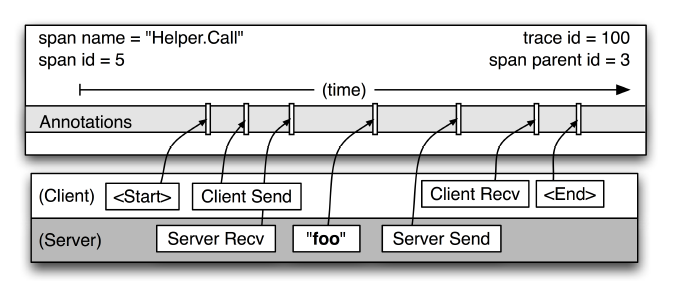
\includegraphics[scale=0.7]{dapper_span.png}
	\caption{Example of Span in Google Dapper. Picture taken from the Google Dapper paper}
	\label{fig:dapper_span}
\end{figure}

Dapper is able to achieve application-level transparency and follow distributed control paths thanks to instrumentation of a few common, mostly shared libraries among Google developers. 
\begin{itemize}
	\item Dapper attaches so called trace-context as thread-local variable to the thread when the thread handles any kind of control path. Trace context is small data structure containing mainly just reference to current and parent span via their ids.
	
	\item Dapper instruments the callback mechanism so when computation is deferred, the callbacks still carry around trace context of the creator and therefore also parent span ans current span id
	
	\item Most of the communication in Google is using single RPC framework with language bindings to different languages. This library was instrumented as well to achieve the desired transparency.
\end{itemize}

Even though Dapper is mainly following black-box monitoring scheme mentioned bellow, it still have small support for adding custom annotation to the code. This gives the developer of an application possibility to attach additional information to spans which are very application-specific.

The low-level overhead was also achieved by sampling the data. As is mentioned in the paper, the volume of data at Google is significant so only samples are taken at a time.

\subsection{Zipkin}
Zipkin is open-source distributed tracing system. It based on Google Dapper technical paper and manages both the collection and lookup of captured data.

Zipkin uses instrumentation and annotations for capturing the data. Some
information are captured automatically such as time when Span was created whereas some are optional and some even application-specific.

Zipkin architecture can bee seen on figure \ref{fig:zipkin_architecture}.
\begin{figure}
	\centering
	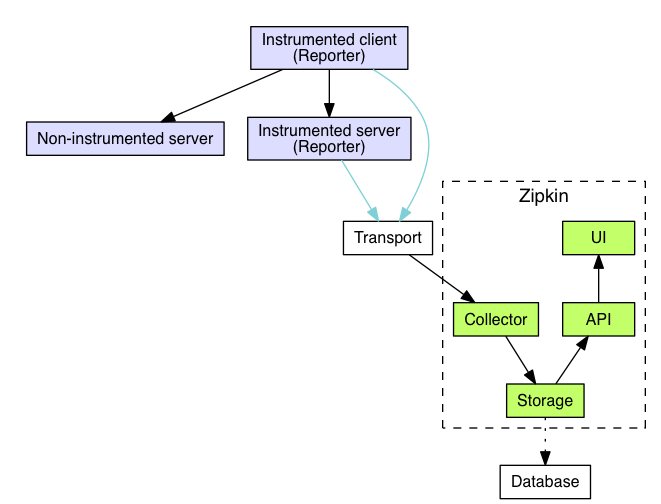
\includegraphics[scale=0.7]{zipkin_architecture.png}
	\caption{Zipkin architecture - http://zipkin.io/pages/architecture.html}
	\label{fig:zipkin_architecture}
\end{figure}
The instrumented application is responsible for creating valid traces. For that reason Zipkin has set of pre-instrumented libraries ready to be used which works well with whole Zipkin infrastructure. Spans are stored asynchronously in Zipkin to ensure lower overhead.

Once the span is created, it is sent to Zipkin, in more details, to Zipkin collector. In General, Zipkin consists of 4 components:
\begin{itemize}
	\item Zipkin Collector
	It is usually a daemon thread or process which stores, validates and indexes the data for future lockups.
	\item Storage
	Data in zipkin can be stored in a mulltiple ways, so this is a pluggable component. Data can be stored in for example in Cassandra, MySQL or can be send to Zipkin UI right away without storing it anywhere. The last option is good only for small amount of data.
	\item Zipkin Query Service
	This component act as a query daemon allowing us to query various informaion about span using simple JSON API.
	\item Web UI
	Basic, but very useful user interface. The user can see whole trace trees and all spans with dependencies between them.
\end{itemize}
 In the thesis the Zipkin UI is used as front end for developed the monitoring tool and it's format is described in more detail in  \hyperref[sec:zipkin_ui]{Zipkin UI} section of \hyperref[chap:design]{Design} chapter.
 
 The reason why Zipkin UI was selected as the primary user interface for this work is mainly it's simplicity and ease of use. Also it fulfills the visualization requirements of the thesis as well, since we need to see dependencies between spans and also whole trace tree as well. However the monitoring platform is not tightly-coupled with this user interface. We will see later how to create custom span savers which can store data in any format suitable for different visualization tools.
 
\section{Background and Tools}
This section covers related tools to the thesis. They are not necessarily used in the thesis, but are important tools used for the monitoring and debugging various kind of applications. The most important tools mentioned in this section are the ones for debugging large scale applications and the profiling tools. We also explain the concept of Flame Graphs as part of the introduction to several profiling techniques. We don't describe visualization techniques in much detail, however Flame Graphs are great concept which may be used for efficient performance analysis, both single and distributed applications.
\subsection{Tools for Large-Scale Debugging}
Standard techniques and tools can be used for debugging distributed applications, however when using these tools we lack the information about dependencies between different nodes in the cluster. There are many tools under the category of large-scale debugging but we just point out basic ideas behind two different approaches - discovering scalling bugs and behaviour based debugging. 

In distributed systems the scalability is very important. It is very important to know how our platform scales when it comes to significantly big data and what is the scalability trend we can expect. It can happen that on large data the platform can run significantly slower than expected when tested on smaller data. We call this issue as a scaling bug. Tools which can be used to help with these kind od bugs are for example Krishna and WuKong. Both of the mention tools are based on the same idea. They build a scaling trend based on data batches of smaller size. The observed scalling trend acts as a boundary. We observe the scalling bug when the scalling trend is violated. In the first tool, Wrishna, we can't tell which port of the program violated the scalling trend, however it is possible in the second tool, WuKong. In comparison to Krishna, Wukong doesn't build one scalling trend of the whole applications, but creates more smaller models, each per some control flow structure in desired programming language where the all these smaller models represent together the whole scalling trend. When we hit into scalling bug, WuKong can give us hints where the trend can be violated.

The different category of tools used for debugging of large scale applications are based on behaviour analysis. The basic idea behind these tools is that the classes of equivalence are created from different program processes and different runs. Using this approach we lower down the number of data we need to inspect and the tools can help us to discover anomalies between different observed classes. For example, STAT - Stack Trace Analysis Tool, is a lightweight and scalable debugging tool used for identifying errors on massive high performance computing platforms. It gathers stack traces from all parallel executions, merges together stacktraces from different processes that have the same calling sequence and based on that creates equivalence classes which make it easier for debugging highly parallel applications. As the other example falling under the same category is AutomaDed. This tool creates several models from an execution and can compare them using clustering algorithm with (dis)-similarity metric to to discover anomalous behaviours. It also can point to specific code region which may be causing the anomaly.

\subsection{Profiling Tools}
Profiling is a form of dynamic code analysis used for analyzing for example how long each part of the system takes in the whole computation, where the computation spends the most time or the memory requirements of the whole program. Generally, we can group the profiling tools into two categories: sampling profilers and instrumentation profilers.

\begin{itemize}
	\item sampling profilers

Sampling profilers take statistical samples of an application at well-defined points such as method invocations. It usually have less overhead comparing to instrumentation profilers. The points were the application should take samples can be inserted at the compilation time by the compiler. Using these profilers we can collect how long the method run, who call it or for example the complete stacktrace. We however can't record any application specific information.
\item instrumentation profilers
This can be solved by instrumentation profilers. These profilers build on the instrumentation of the application's source code. They record the same kind of information as the sampling profilers but usually give us the ability to specify extra points in the code we are interested in and also to record application specific data.
\end{itemize}


However, we can look on profilers from different point of view and categorize them based on the level on which they operate and are able to record the information - system profilers and application specific profilers. 
At application specific profilers, we are the most interested in profilers targeted for JVM platform.
\begin{itemize}
	\item system profilers
	System profilers operate on OS-level. They are great at showing system code paths, but are not able to capture method calls done for example in Java application.
	\item JVM profilers
	These profilers show Java methods, but usually not system code paths.
\end{itemize}
The ideal solution for monitoring purposes would be to have information from both kind of profilers, however combining outputs of these profiler types is not straightforward. The profilers which are able to collect traces from both the profiler types are usually called mixed-mode profilers. JDK8u60 comes with the solution in a way of extra JVM argument \textit{-XX:+PreserveFramePointer} \cite{MixedModeProfilers}.  Operating system is usually using this field to point to most recent call of the stack frame and system profilers make uses of this field. In case of Java, compilers and virtual machines don't need to use this field since they are able to calculate the offset of the latest stack frame from the stack pointer. This leaves this register available for various kind of JVM optimalizations.

This option ensures that JVM abides the frame pointer register and will not use it as general purpose register and therefore we can get both system and JVM stack frames in a one call hierarchy. Using the JVM mixed-mode profilers we are able to collect information about:
\begin{itemize}
	\item page faults
	They allow us to see what leads to from of JVM resident memory.
	\item context switches
	Context switches are interesting to see code path leads to leaving the CPU.
	\item disk i/o requests
	Show code paths leading to IO operations such as blocking disk seek operation.
	\item TCP events
	Show code paths leading from high-level Java code to low-level system methods such as connect or accept, so we can reason about performance and good design of network communication in much more better detail.
	\item CPU cache misses
	Show code paths leading to cache misses. Using this information we can optimize the Java code to make better use of the existing cache hierarchy.
\end{itemize}

All the information bellow can be described on a special chart called Flame charts.
\subsubsection{Flame Charts}
Flame Chart is a concept by a developer Brendan Gregg. Flame graphs are aa visualization for samples stack traces, which allows the hot paths in the code to be identified quickly. The output of sampling of instrumentation profiler can be significantly big and therefore visualizing can help to reason about performance in more comfortable way. 

\begin{figure}
	\centering
	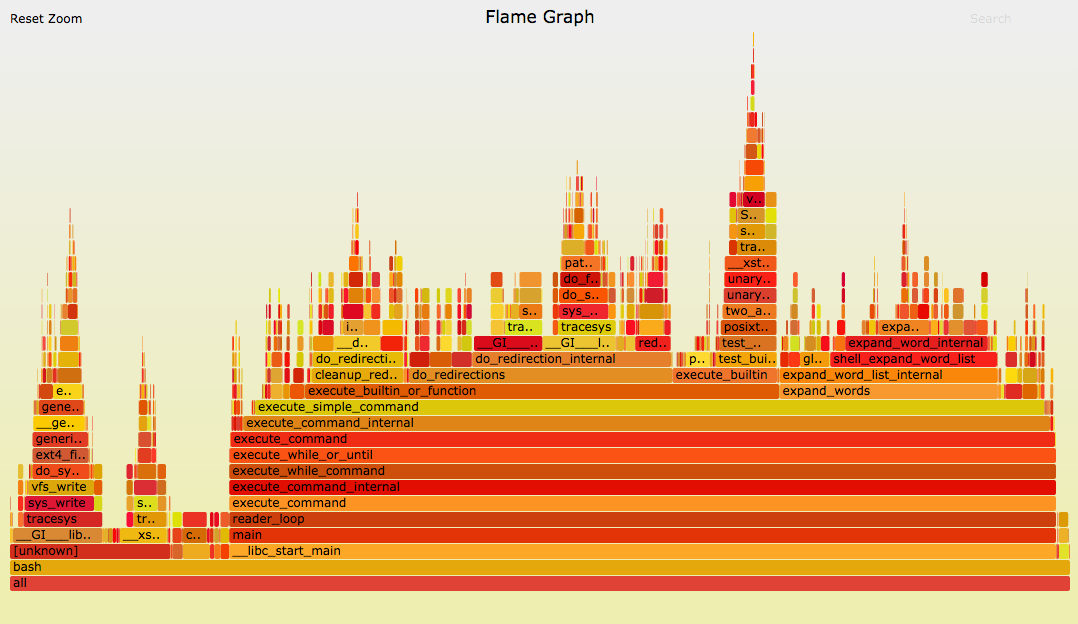
\includegraphics[scale=0.35]{flame_chart.png}
	\caption{Flame Graph example}
	\label{fig:flame_chart}
\end{figure}
The description:
\begin{itemize}
	\item Each box represents a function call in the stack
	\item The \textbf{y-axis} shows stack frame depth. The top function is the function which was at the moment of capturing this flame chart on the CPU. All functions underneath of it are its ancestors.
	\item The \textbf{x-axis} shows the population of traces. It doesn't represent passing of time. The function calls are usually sorted alphabetically.
	\item The width of each box represents the time the function was on CPU.
	\item The colors are not significant, they are just used to visually separate different function calls
\end{itemize}

Flame charts can be created in a few simple steps, but it depends on the type of profiler the user wants to use. 
\begin{enumerate}
	\item Capture stack traces
	For this step we can use profiler of our choice.
	\item Fold stacks
	We need to prepare the stacks so Flame graphs can be created out of them. For this, there are several scripts prepared for different profiler types.
	\item Generate the flame graph itself, again using the prepared script provided on the link above.
\end{enumerate}

Purpose of this really short section was just to introduce the idea of Flame charts since it's one of the future plans the thesis could be extended to support. For more information about the flame charts please visit the Brendan Gregg's blog.

\section{Instrumentation Libraries}
\subsection{Javassist}
\subsection{ByteBuddy}
\subsection{CGlib}
\subsection{ASM}
.. just give brief overview what were the instrumentation libreries choices. The selected one will be describied in the next section

\section{Communication Middleware}
give comparison between the possible communication middle-wares
\subsection{Raw Sockets}
\subsection{ZeroMQ}
\subsection{NanoMSG}

\section{Comparison of Agent Approaches}
give introduction to various instrumentation techniques and compare the 2 approaches
\subsection{Java Agent Solution}
\subsection{Native Agent Solution}


\chapter{Design}
\label{chap:design}
This chapter describes design of the whole platform in details, however implementation specifics of some parts of the tool are described in the following chapter.  This chapter starts with an high-level overview of the complete platform and interactions between the parts and follows by a simple use-case to give the reader idea how this tool is mean to be used. 

Spans and their format are described next followed by design of the native agent and instrumentation server. This chapter ends by describing the used Zipkin user interface and also JSON format in which the user interface accepts the data from the instrumentation server. 

\section{Overview}
Main purpose of this tool is to collect distributed traces. In order to achieve that, the thesis is based on the concept of Spans. Spans are used to denote some specific part of the communication between the communicating nodes and are the important elements for building the whole trace trees. Trace trees consists of several spans and represent the complete task or communication where a span inside the trace represents usually a few remote procedure calls between two neighboring nodes. The node initiating the trace creates so called parent span and new calls started within this span create new nested spans. Created spans can be processed using different span savers and can be send to the user interface using various data collectors. 

Spans are processed using Span Savers. Span savers are used to save spans in desired format on disk or on the network for further data collection and collected data are used for Spans visualizations in the user interface. The user interface receives the spans from the span savers or data collectors and present them to the user in a form of trace trees.

Definition of when a new span is to be created and when an existing span needs to be closed is done by a developer by extending the core instrumentation server library. The created instrumentation server is then used for instrumenting the classes of the original application at which information about spans needs to be preserved. In order to obtain the class files, the native agent runs  as part of the monitored application and sends the instrumentation server the desired classes. The native agent is the core part of the whole platform. It is attached to the monitored application and additionally to the instrumentation, it is used to obtain various low-level information from the application. 

The tool therefore consists of three main parts:
\begin{itemize}
	\item Native Agent
	\begin{itemize}
		\item Is used to obtain byte-code for the instrumentation
		\item Is used to actually apply the instrumented byte-code
	\end{itemize}
	\item Instrumentation Server
	\begin{itemize}
		\item Instruments the classes obtained from the native agent
		\item Is also a base library for custom application instrumentation server
		\item Can contain implementations of custom span savers
	\end{itemize}
	\item User Interface
\end{itemize}


The graph \ref{fig:architecture} denotes the basic relationships between the major parts. Each part is explained in more detail later in this chapter. \begin{figure}
	\centering
	
\includegraphics[scale=0.6]{architecture.png}
	\caption{Basic relationship between the major components. Instrumentation server communicates with the native again mainly in order to instrument classes. The Application's communicates with the user interface by sending the spans. Spans can be send either via data collection agent or one of the default span savers explained later in this chapter.}
	\label{fig:architecture}
\end{figure}

\section{Example Use Case}
TODO: write proper small example!

In order to have a better understanding how this platform can be used we provide simple example of client-server application as an use-case, so far without the code. Clients query the server and server provides them with the response. We would like to instrument the client and the server and monitor the communication between the client and the server.

Because client and the server are different applications, we need to create 2 different instrumentation servers and specify what is the method and a class which is required to be instrumented and what should happen in the instrumented code. In this case we just want to add custom annotations to recorded spans which are specific to the client-server communications.

The native agent has to be attached to both the client and the server prior it's start and the path to the instrumentation server jar needs to be set on both client and server to corresponding server. The default span sever is used in this case and the collected spans are send right to the Zipkin UI. The default endpoint for the user interface is used when not defined as an argument to the native agent.

We can see that the only part the user needs to worry about is the extension of the instrumentation server to specify the custom instrumentation points, otherwise the rest of the work is done automatically.

\section{Spans and Trace Trees}
\label{subsec:spans}
As mentioned briefly in the previous section, spans are used to gather the information about the distributed calls or so called, distributed stack traces. Points in the code where spans are created and closed are defined as part of the Instrumentation server but since it's the most important concept in the thesis, we explain them in the separated section. 

Spans are the main concept behind capturing the distributed traces. They are special classes which instances are injected to instrumented application's classes to keep track of the communication and the state between the nodes in the distributed application. Usually, the initiator creates so called parent span and new calls started within the span create new nested spans. Collected spans can be processed using different span savers and can be sent to the user interface using various data collectors.

Spans has several mandatory and optional fields. The mandatory fields are trace id, span id and parent span id. Trace id represents one complete distributed call among all interacting nodes on the cluster. This field is attached automatically when a new root span is created. Root span is a first span created inside a trace. The root span does not have parent id field set up and therefore the user interface back-end can distinguish between regular spans and root spans and therefore can identify the start of the whole trace. Parent id of a span is always id of span from which the span received a request to perform some task. The span and its parent span can be located on the same node or on different nodes as well. The first variant can be useful in cases where the developer requires to trace several threads as separated spans within a single node.  

Span have several additional fields which which are later used in the user interface. The fields are:
\begin{itemize}
	\item \textbf{Timestamp} - when the span started.
	\item \textbf{Duration} - how long the span lasted.
	\item \textbf{Annotations} - annotations which are used to carry additional timing information about spans. For example time when span has been received on the receiver side or the time the span has been processed at the receiver side can be set using the annotations.
	\item \textbf{Binary annotations} - annotations which can be used to carry around application specific details. We can use these annotations to transfer information between communication nodes inside of spans. For example, one node can store number of bytes sent during the request and the receiver can use this information to calculate overall number of bytes received from this particular node.
\end{itemize}

Each annotation, both binary and regular, has also endpoint information attached. This element consist of:
\begin{itemize}
	\item \textbf{ip} - ip of the node on which this event was recorded
	\item \textbf{port} - port on which the service which recorded the span is running.
	\item \textbf{service name} - service name which is used to group different traces by names and can be later used to filter traces using this field in the user interface.
\end{itemize}

The following sections contains information about how spans are exported for external communication with the user interface and also how spans are created using \texttt{TraceContext} and \texttt{TraceContextManager} classes.
\subsection{Span Savers \& Data Collectors}
Spans are exported from the application using the span savers. Span saver for the application may be selected via one of the native agent configuration properties. It is important to mention that all spans in the application are using the same, because span saver is static field of the \texttt{Span} class. Span savers need to be available to the monitored application and therfore are brought to the application from the instrumentation server via the native agent during the agent initialization phase.

The thesis provides two default implementation of span savers but also allows the developer to create new span savers. New span savers may be useful in cases when the developer wants to export the span data in a format used by different user interface or to use custom data collector. Data collector is a service which collects the data from the specified place and store them in central data storage available by all application's node. This thesis does not implement data collection service as many services exists for this purpose. 

Data collected within spans are internally represented in JSON format understandable by the Zipkin user interface. This is also the reason why the thesis contains support for working with JSON data and  it is explained in more detail later in the  \hyperref[chap:implementation]{Implementation} chapter. This format can be again changed by the custom span saver.

Span saver implementations need to extend from the abstract ancestor defining common methods for each span saver. Also, in order to be able to use the saver automatically in the code, it has to have a constructor with single \texttt{String} argument accepting saver arguments. The arguments format is defined in the case of default span savers however the developer may use any format in case of custom span savers. The common ancestor, \texttt{SpanSaver} abstract class has two abstract methods:
\begin{itemize}
	\item \texttt{saveSpan}. This method is used for saving the span. Custom span saver implementation may save the data on local disk or send over network. The destination is not limited by the code. Internally, this method is called asynchronously in a separated thread to allow asynchronous span processing which has a performance benefit.
	\item \texttt{parseAndSetArgs}. The instrumentation agent accepts also special argument which contains arguments for the defined span saver. Each span saver is responsible for parsing the span saver arguments.
\end{itemize}

As mentioned above, the tool provides two default simple span savers:
\begin{itemize}
	\item  \texttt{DirectZipkinSaver} - The default span saver sends the collected span  asynchronously to the user interface right away without storing the data on disk to be collected by an external data collector. In this case the functionality of the span saver and the data collector are handled by this single saver. This span saver should be used for demonstration purposes only since it could overload the user interface or network when processing and sending high amount of collected spans in a short amount of time to the user interface as the UI is not prepared to store large amounts of data in the memory. 
	
	This saver accepts a single argument which is ip and port of the Zipkin UI service. The diagram \ref{fig:zipkin_span_saver} shows how the Zipkin span saver is used.
	
		\begin{figure}
			\centering
			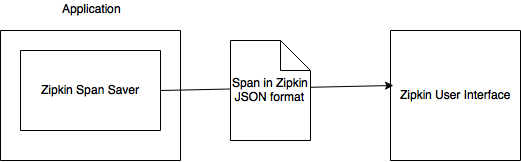
\includegraphics[scale=0.6]{zipkin_span_saver.png}
			\caption{Using the Zipkin span saver to save spans directly to Zipkin user interface without the data collector agent.}
			\label{fig:zipkin_span_saver}
		\end{figure}
	\item  \texttt{JSONDiskSaver} - The second available span saver saves the collected data asynchronously on disk in the format known to Zipkin UI for future collection to the Zipkin user interface by custom data collector. Together with some well-known data collection agent, this is a preferred way of transferring spans from the application to the Zipkin user interface in the production. This saver accepts single argument which is a directory where collected spans are saved. The diagram \ref{fig:disk_span_saver} shows how JSON disk span saver is used.
	\begin{figure}
		\centering
		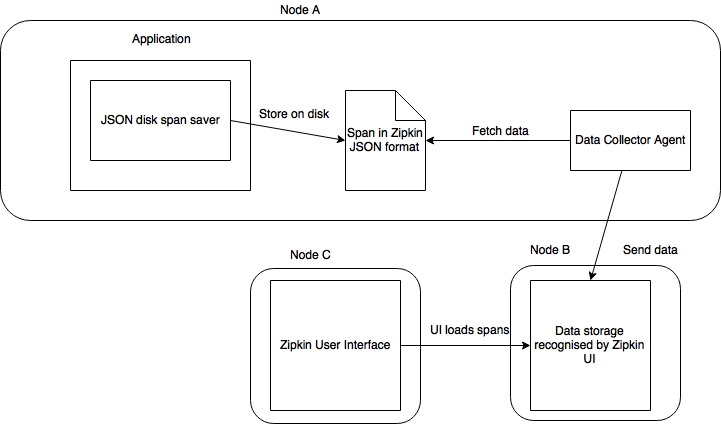
\includegraphics[scale=0.5]{disk_span_saver.png}
		\caption{Using the JSON disk saver together with the data collection service but Zipkin user interface .}
		\label{fig:disk_span_saver}
	\end{figure}
\end{itemize}
Additionally, the diagram \ref{fig:custom_span_saver} shows how a custom span saver may be used.

\begin{figure}
	\centering
	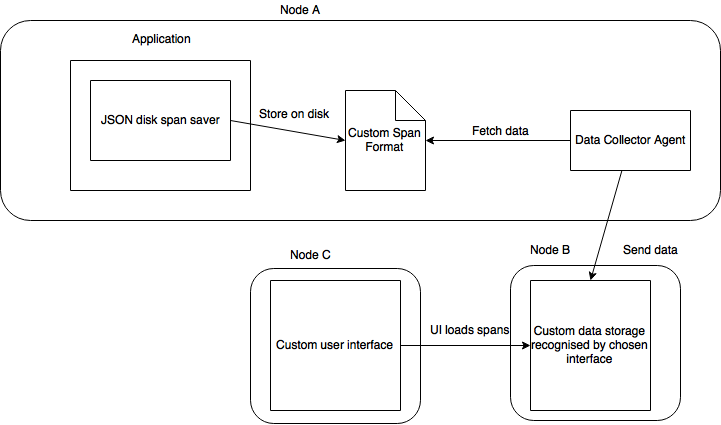
\includegraphics[scale=0.5]{custom_span_saver.png}
	\caption{Using custom span saver together with the data collection service and custom user interface.}
	\label{fig:custom_span_saver}
\end{figure}
In order to give the developer the flexibility to add new savers without changing the internals, the span savers have to be  registered in the META-INF directory of the extended instrumentation server JAR file. This ensures that the service loader can find all implementations of the \texttt{SpanSaver} abstract class. The reason why the classes needs to be discovered is explained in the following \hyperref[native_agent_design]{Native Agent} section. 

To make the developer life easier, the \textbf{AutoService} library from \textit{https://github.com/google/auto/tree/master/service} is used. Instead of manually registering the implemented span savers into META-INF directory, they can be annotated in the code using the \texttt{AutoService} annotation with a single argument specifying the abstract parent, in this case \texttt{SpanSaver}. The library takes care of registering the classes automatically in the desired folder in correct format so the human error is minimized.

\subsection{Trace Context}
Trace context is a class used for storing the information about the current span and also for creating new spans and closing current spans. Trace context is always attached to a specific thread. This is done in order to allow multiple threads to have different computation state and therefore the platform is able to capture multiple distributed traces at the same time on the same node. Singleton instance of class \texttt{TraceContextManager} is used for attaching the threads to the trace contexts and vice-versa. It has a few methods allowing the developer to attach trace context to a specific thread and also to get trace context which is attached to a current thread.

Each trace represented by a trace context is uniquely identified by \texttt{Universally unique identifier (UUID)} of type one is created. This UUID version combines 48-bit MAC address of the current device with the current timestamp. This way it is ensured that two traces created at the same time on different nodes can't have the same identifier. The identifiers are created using a C++ library called sole (https://github.com/r-lyeh/sole) in the native agent and are made available to the Java code via a published native method.

The trace contact has method s\texttt{openNestedSpan} and \texttt{closeCurrentSpan}. The first method is used to create a new nested span and set the newly created span as the current one. Nested span is a span which sets its parent id to the current span. A root span is created in case when no current span exists. The second method is used to close the current span. Closing the span triggers the span saving operation on the used span saver and the parent span becomes the current span.

The diagram \ref{fig:closing_spans} shows how spans are created, closed and saved.  in this chapter. \begin{figure}
	\centering
	
\includegraphics[scale=0.6]{closing_spans.png}
	\caption{Creating and closing spans.}
	\label{fig:closing_spans}
\end{figure}

\section{Native Agent}
\label{native_agent_design}
The native agent is used for accessing the internal state of the monitored application and also to instrument classes so they can carry the span and trace identifiers between the application nodes. The main agent task is to check whether a class is required to be instrumented and if yes, send the class for the instrumentation to the instrumentation server and wait for the instrumented code.

The native agent consist of several parts. The most important parts are:
\begin{itemize}
	\item \textbf{Bytecode parsing module}. \newline The classes in this module are used to parse the JVM byte code in order to discover the classes dependencies for further instrumentation. Byte code parsing is a technical task described in the following \hyperref[chap:implementation]f{Implementation} chapter.
	\item \textbf{InstrumentorAPI}. \newline The \texttt{InstrumentorApi} class provides several methods which are used to communicate with the instrumentation server JVM. All the queries to the server are done via instance of this class.
	\item \textbf{AgentCallbacks}. \newline All callbacks used in the native agent are defined in this namespace.
	\item \textbf{AgentArgs}.  \newline The \texttt{AgentArgs} class contains all the logic required for argument parsing.
	\item \textbf{NativeMethodsHelper}. \newline The \texttt{NativeMethodsHelper} class is used for registering native methods defined in C++. These methods can be later used from the Java code without worrying of the low-level implementation.
	\item \textbf{Utilities module}. \newline This module contain several utility namespaces. The most important utility namespaces are \texttt{AgentUtils} and \texttt{JavaUtils}. The first one contains methods for managing the JVMTI connection and for registering the JVMTI callbacks and events. The second one is used to simplify work with Java objects in the native code via JNI. 
\end{itemize}

\subsection{Agent Initialization}
The agent is initialized via the same phases as described in the \hyperref[subsec:jvmti_init]{JVMTI Agent Initialization}  section of the \hyperref[chap:background]{Background} chapter. The following JVMTI events are especially important to the thesis: \texttt{VM Init}, \texttt{VM Start}, \texttt{VM Death}, \texttt{Class File load Hook}, \texttt{Class Prepare} and \texttt{Class Load}. Callbacks are registered for all the mentioned events so the native agent can react to them accordingly in the code.

As part of the initialization process, the agent is responsible for either connecting to or starting a new instrumentation server. In case the native agent was started in the shared mode of the instrumentation server, the agent tries to connect to already existing server and the server is shared between all application's nodes. In the local instrumentation mode, the instrumentation server is started as a separated process automatically and the connection is established with the server using the inter process communication. In this case, each application node has dedicated instrumentation server.

The callback registered for the \texttt{VM Init} event is responsible for loading all additional classes from the instrumentation server as part of the initialization as well. The additional classes are for example \texttt{Span}, \texttt{TraceContext} or custom implementations of \texttt{SpanSaver} abstract class. These classes are used in the instrumented code and therefore have to be available to the monitored application. The native agent is designed in a way that developers are not supposed to change the code of if. All the extension are supposed to be done within the instrumentation server. Therefore, the instrumentation server is asked at the initialization phase for the list of all additional classes and they are sent to the native agent. The agent puts all the received classes on the application's class-path so they are available to the instrumented code.

\subsection{Instrumentation}
Code for handling the instrumentation is part of the callback for the \texttt{Class File load Hook} event. The callback has the byte code for the class being loaded as its input parameter and allow the developer to pass a new instrumented byte code as the output parameter. The process of instrumentation is described here, however the technical details are described in the following chapter.

The process consist of several stages:
\begin{enumerate}
	
	\item Enter the critical section. It can happen that the class file load hook is triggered multiple times and in order to not confuse the instrumentation server, the lock has to be acquired before the instrumentation of a class starts.
	\item Firstly, the check whether the virtual machine is started is done. If the virtual machine is started and initialized, the instrumentation continues, otherwise the instrumentation for currently loaded class is skipped without asking the instrumentation server since it the class is a system class and it is not desired to instrument Java system classes at this moment.
	\item Attach JNI environment to the current thread. Since the JVMTI and JNI does not have automatic thread management, it's up to the developer to take care of correct threading management.
	\item Discover the class-loader used for loading the class
	\item Parse the name of the class being loaded. Even though the callback provides input parameter which should contain the name of loaded class, at some circumstances it can be set to \texttt{NULL} even though the class name is available in the byte code. Instead of relying on this parameter, the byte code is parsed and the class name is found manually.
	\item Decide whether the instrumentation should continue. This check is based on the used class loader and name of the class being loaded. Classes loaded by the \texttt{Boostrap} class loader and in case of Sun JVM, from \texttt{sun.reflect.DelegatingClassloader} are not supposed to be instrumented. 
	The \texttt{Boostrap} class loader is used to load system class and the second mentioned class loader is used to load synthetic classes and in both cases, it's not desired to instrument classes loaded by these class loaders.
	There are also some ignored classes for which the instrumentation is not desired. Example of these classes are the classes loaded during initialization phase from the instrumentation server and the auxiliary classes generated by the Byte Buddy framework. Auxiliary classes are small helper classes Byte Buddy is using for instance for accessing the super class of the currently instrumented class. Therefore the instrumentation continues only If the class is not ignored and not loaded by ignored class loader.
	\item The instrumentation server is asked whether it already contains the loaded class or not and also if the class should be instrumented. The agent does not know which classes are to be instrumented and it therefore needs to query the server. The classes for instrumentation are marked by developer when extending the instrumentation server library using simple Byte Buddy API. 
	
	If the server does not contain the class, the native agent sends the class data to the instrumentation server, parse the class file for all the dependent classes and send all dependent classes to the instrumentation. This step is repeated throughout the dependency scan recurrently until the loaded class does not have any other dependencies or until all dependencies is already available on the server. All dependencies for the currently instrumented class have to be available on the server in order to perform the instrumentation.

	\item At this stage, the class is already on the instrumentation server and all dependencies for this class as well. The native agent waits for the instrumented byte code to be send from the server. 
	\item Exit the critical section.
\end{enumerate}	
Even though the class is fully instrumented and the instrumented byte-code is available to the agent, the process is not completely done. The instrumentation library used at the instrumentation sever ( Byte Buddy) is using so called \texttt{Initializer} class to set up special interceptor field in the instrumented classes. It is a static field which references the instance of the class interceptor - class defining the instrumentation code. This field is automatically set by Byte Buddy framework in most of the cases, but since in case of this thesis the instrumentation is done on different JVM then where the code is actually running, it needs to be handled explicitly. In order to set this field by corresponding \texttt{Initializer} class, both the initializer class and interceptor class need to be available on the agent. The instrumentation server sends the initializer class together with the instance of interceptor during the instrumentation of the class and the agent registers the interceptor and initializers with the instrumented class for later use since the static interceptor field can be set up when the class is used for the first time. The initializers are loaded during  \texttt{Class Prepare} event. This event is triggered when the class is prepared but no code has been execute so for. 

The callback for \texttt{Prepare} event is also used to register the native methods for the class being loaded. Registering the native method to the class makes it available from Java programming language.

Several technical difficulties had to be dealt with during the development. For example,  cyclic dependencies when instrumenting the class had to be properly handled. Also ensuring that the dependencies for the instrumented class are also instrumented in the correct order has been a significant challenge. The different attempts for the solution and the final solution is described in the following chapter since it's highly implementation specific.
\subsection{Instrumentation API}
The Instrumentation API is used to communicate with the instrumentation server. It provides low-level methods for sending data in form of byte arrays or strings and the corresponding methods for receiving the data. On top of these method several methods are built to make the communication easier. The most important methods are:
\begin{itemize}
	\item \texttt{sendClassData} method sends byte code to the instrumentation server.
	\item \texttt{isClassOnInstrumentor} method checks whether the byte code for the given class is already on the instrumentation server or not.
	\item \texttt{instrument} method triggers the instrumentation and returns the instrumented byte code.
	\item \texttt{loadInitializersFor} method is for loading the initializers for specific class.
	\item \texttt{loadDependencies} method is used to load all dependent classes and upload them on the instrumentation server. The dependency is uploaded only in case it's not already available on the instrumentation server.
	\item \texttt{shouldContinue} method checks if the class on its input is allowed to be instrumented.
	\item \texttt{loadPrepClasses} method loads all dependent classes in the agent initialization phase.
\end{itemize}

\subsection{Native Agent Arguments}
The native agent accepts several arguments which can be used to affect the agent behavior. In local instrumentation server mode, several arguments affect also the sever started from the agent. Available arguments are:
\begin{itemize}
	\item \textbf{instrumentor\_server\_jar} - specifies the path to the instrumentation server JAR. It is a mandatory argument in case the instrumentation server is supposed to run per each node of monitored application.
	\item \textbf{instrumentor\_server\_cp} - specifies the classpath for the instrumentation server. It can be used to add application specific classes on the server classpath which has the effect that the monitored application does not have to send to the server these classes if they need to be instrumented or if some class to be instrumented depends on them.
	\item \textbf{instrumentor\_main\_class} - specifies the main entry point for the instrumentation server. It is a required argument in case of local instrumentation server mode.
	\item \textbf{connection\_str} - specifies the type of connection between native agent and the instrumentation server. It is a mandatory argument in shared instrumentation server mode in which case the value is in format \texttt{tcp://ip:port} where ip:port is address of the instrumentation server. Otherwise, the agent and server communicates via inter-process communication and the argument can be set in format \texttt{ipc://identifier} where identifier specifies the name of pipe in case of Windows and name of the file used for IPC in case of Unix. However this value is set automatically at run-time if not explicitly specified as an argument.
	\item \textbf{log\_dir} - specifies the log directory for the agent and when running in local server mode, specifies the log directory for the server as well.
	\item \textbf{log\_level} - specifies the log level for the agent and when running in local server mode, specifies the log level for the server as well.
	\item \textbf{saver} - specifies the span saver type. The value can be either \texttt{directZipkin(ip:port)} where ip:port is address of the Zipkin UI interface or \texttt{disk(destination)} where destination sets the output directory for the captured spans. Custom span savers are supported as well. In that case the format of the value is a fully qualified name of the span saver with arguments in parenthesis, for example as \texttt{com.span.saver(arguments)}
	\item \textbf{config\_file} - specifies path to a configuration file containing the agent configuration. It can contain all arguments mentioned above, each argument per one line of the configuration file.
\end{itemize}

\section{Instrumentation Server}
\label{sec:inst_server}
The instrumentation server is responsible for instrumenting the byte code received from the native agent in separated JVM and also acts as the base library for the instrumentation for specific applications. The developer extending the instrumentation server can use prepared method to define custom instrumentation points without touching the internals of the native agent.

This section covers several design aspects of the instrumentation server, leaving the implementation details on the following sections. The core instrumentation on the server is handled by the Byte Buddy code manipulation framework. The native agent asks the server if the class being loaded is required to be instrumented. If yes, the server receives the byte code, performs the instrumentation and sends the data back to the agent. The server does not contain any application state, in particular it does not take track about the distributed traces. The information about traces is contained in the application's instrumented classes.

The platform was designed to be configurable and deployment of instrumentation server is supported via two approaches. The instrumentation server can be either on the network available to all the application nodes and can be shared by all applications. This has the advantage of caching the instrumented classes. So when any class is instrumented for the first time, it is saved and the instrumentation is not performed for other nodes but the class is immediately sent. The disadvantage of this solution is higher latency between the agent and the instrumentation server since they are usually not on the same node. In this case the instrumentation server has to be manually started in advance. Architecture of this scenario is depicted on the diagram \ref{fig:shared_server}.
 
 \begin{figure}
 	\centering
 	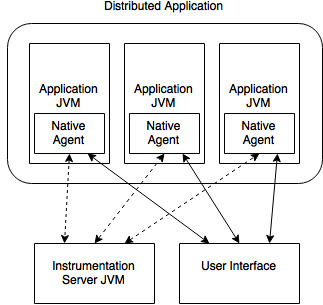
\includegraphics[scale=0.8]{shared_server.png}
 	\caption{Architecture with shared instrumentation server. The dotted lines represents the communication between instrumentation server and the agent whilst the regular lines represents data collection from the agent to the UI}
 	\label{fig:shared_server}
 \end{figure}
 
 The other deployment method is that the instrumentation server runs on each application node. This has the advantage of faster communication since  inter-process communication is used to communicate between monitored JVM and the instrumentation server. The disadvantage of this solution is that all classes have to be instrumented on each node since there is no communication between the instrumentation servers. In this solution, the server is started automatically during the native agent initialization. Architecture of this scenario is depicted on the diagram \ref{fig:separated_server}.
 
 \begin{figure}
 	\centering
 	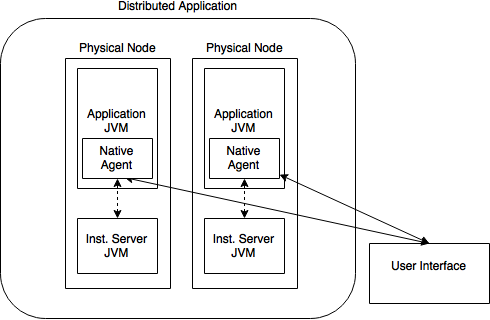
\includegraphics[scale=0.8]{separated_server.png}
 	\caption{Architecture with separated instrumentation server. The meaning of the lines is the same as on the diagram above.}
 	\label{fig:separated_server}
 \end{figure}

Except from the cached classes, the server does not contain any application state and it just reacts to the agent requests. It can accept four type of requests:
\begin{itemize}
	\item Request for code instrumentation.
	\item Request for storing byte code for a class on the server.
	\item Request for sending all helper classes needed by the agent such as the \texttt{Span} class or \texttt{TraceContext} class.
	\item Request to check whether the server contains specific class or not.
\end{itemize}
The server interacts in more ways with the agent, however they are just sub-parts of the communication initiated by one of these 4 request types.	

The instrumentation server needs to deal with several technical problems. The main issue is that the classes which are about to be instrumented require all other dependent classes to be available. The other issue is instrumenting the classes with circular dependencies. The server also performs several optimizations to provide faster response to the agent such as caching the instrumented classes or minimizing the communication when possible. The technical aspects of these issues and the optimizations mentioned above are described in the following sections.
\subsection{Instrumentation}
The instrumentation of the class is triggered by the agent and it's done in two stages. The first stage informs the client whether the class is already on the instrumentation server or not. The second stage is the instrumentation itself. The first stage is initiated by the agent. The server performs the check for class availability in 3 phases:
\begin{enumerate}
	\item Check whether the instrumented byte code for this class is available.
	\item If not, check whether the original byte code for this class is available.
	\item If not, check if the class can be loaded using the server's context class loader. This handles the cases where the user builds the instrumentation server together with the application classes or adds the application classes on the instrumentation server classpath for optimization reasons.
\end{enumerate}

The server informs the agent if it does not have the byte code for the class available and in that case  the agent sends the class to the server. The server registers the received byte-code under the class name. The agent therefore does not have to send the class next time since it's already cached on the instrumentation server.
The second stage follows the first stage immediately. If the server already contains the instrumented class in the cache, the instrumented class is sent right away without instrumenting the class again. If the cache is empty, the class is instrumented and put into the cache.

The code instrumentation is handled by \texttt{CustomAgentBuilder} and \texttt{BaseAgentBuilder} classes.
The instrumentation server expects instance of \texttt{CustomAgentbuilder} on the input of its \texttt{start} method. This is an abstract class containing single abstract method \texttt{createAgent(BaseAgentBuilder builder, String pathToGeneratedClasses)} where the builder is a wrapper around the Byte Buddy \texttt{AgentBuilder} class which is used to define the class transformers.

The developer needs to implement this method and specify on which classes and on which methods the instrumentation should happen. Since Byte Buddy is used for writing transformers and interceptors, please read more about Byte Buddy in the \hyperref[sec:byte_buddy]{Byte Buddy} section. The server provides several helper methods for creating the transformers and interceptors which are less verbose then the standard Byte Buddy approaches.

Each created transformer has to have associated `n interceptor which defines the code to be injected. Each interceptor implementation has to implement \texttt{Interceptor}  interface. This is required for the server to be able to discover all interceptors at run-time without the need for changing the internals of the server. Each implementation of the interceptor needs to register itself in the META-INF directory of the generated JAR in the same way as the span savers mentioned in the previous section. Custom service loader is then used to locate all classes implementing the \texttt{Interceptor} interface.

Even though Byte Buddy takes care about the instrumentation, the \texttt{BaseAgentBuilder} class is internally properly configured so the instrumentation happens exactly as desired. The class implements four Byte Buddy listeners used for informing us about the instrumentation progress and allow us to react on the process of the instrumentation. The listeners are:
\begin{itemize}
	\item \texttt{onTransformation} listener is called immediately before the class is instrumented.  Implementation of the listener in the thesis also sends the agent all auxiliary classes required by the instrumented class and the initializers used for setting the static interceptor field on the instrumented class.
	\item \texttt{onIgnored} listener is called when the class is not instrumented. The class is not instrumented when the user does not define any transformer for the specified class.
	\item \texttt{onError} listener is called when some exception occurred during the instrumentation.
	\item \texttt{onComplete} listener is called when instrumentation process completed. It is called after both of \texttt{onTransformation} and \texttt{onIgnored} listeners.
\end{itemize}

Byte buddy requires dependencies for the instrumented class to be available. They are needed because the instrumentation framework needs to know signature of all methods in several cases, for example when the method is overridden in the child class. The dependencies are all the classes specified in the class file such as type of the methods return value or arguments, super class or implemented interfaces. 
By default, Byte Buddy tries to find these dependencies using two classes - \texttt{LocationStrategy} and \texttt{PoolStrategy}. The first class is used to tell Byte Buddy where to look for the raw byte code of dependent classes. The classes are loaded by context class loader by default, but since the classes are received over the network, custom \texttt{InstrumentorClassloader} class loader is used to handle the class loading. It is a simple class loader which keeps the cache of the classes received from the agent and when a request for instrumentation comes, instead of looking into the class files, it loads the data from the cache in the memory.

However, Byte Buddy internal API does not work with raw byte code for scanning the further dependencies and obtaining the metadata for the classes. It uses classes \texttt{TypeDescription} and \texttt{PoolStrategy} for this purpose. The first class has a constructor accepting the \texttt{Class} class and created instance contains metadata for the class such as the signature of all methods and fields, list of all interfaces or for example list of constructors. The second class is used for caching the type descriptions so they are not created every time the class is accessed. 

So in overall, class lookup is done in the following two steps:
\begin{enumerate}
	\item Check whether type description for the class is available. If yes, load the type description from the cache.
	\item If the type description is not available, load the class using the \newline \texttt{InstrumentorClassloader}, create type description for the class and put it in the cache.
\end{enumerate}

\subsection{Custom Service Loader}
In order to allow the developer to extend the base instrumentation library service loaders for loading the extensions are used. The service loader is used used for two types: 
\begin{itemize}
	\item Custom span savers. Each span saver inherits from the abstract class \texttt{SpanSaver}.
	\item Custom Interceptors. Each interceptor implements the interface \texttt{Interceptor}.
\end{itemize} 
The user can create custom span savers and interceptors by either inheriting the desired class or implementing the required interface and put the name of the class inside the text file in the META-INF directory in the JAR file. The text file has to have tha same name as the abstract class or the interface the implementation is for. For example, when user creates a new Interceptor called \texttt{x.y.InterceptorA}, the file \texttt{Interceptor} in the META-INF folder has to contain line \textbf{x.y.InterceptorA}.

Java provides service loader for this purpose. However the standard Java implementation looks up the classes defined as above and automatically creates new instances using the well-known constructors. For the thesis purposes this was unwanted as it's only required to obrain \texttt{Class} object representing the available implementation. Therefore a custom service loader was created for this purpose. This loader works in very similar way as the standard Java one, but instead of returning the instances of loaded services it just returns classes of available services. 

\subsection{JSON Generation}
The data inside spans are internally stored as instances of \texttt{JSONValue} class since in order to support the communication with the default Zipkin UI they need to be exported as JSON. JSON is a lightweight format for exchanging data where the syntax is based on Javascript object notation.

The JSON handling is based on the https://github.com/ralfstx/minimal-json library, however custom simplified implementation was created which fits the theses requirements. Also the number of dependencies is lowered by this decision. 

This JSON support is designed via several classes:
\begin{enumerate}
	\item \textbf{JSONValue}. The abstract ancestor of all JSON types. This type defines common methods to all implementation.
	\item \textbf{JSONString}. Class representing the string type.
	\item \textbf{JSONNumber}. Class representing the numeric types.
	\item \textbf{JSONLiteral}. Class representing the literals \textbf{null}, \textbf{true} and \textbf{false}.
	\item \textbf{JSONArray}. Class representing the JSON arrays. It has support for adding new elements into the array.
	\item \textbf{JSONObject}. Class representing the JSON objects. It has support for adding a new items in the object.
\end{enumerate}

Each \textbf{JSONValue} can be printed as valid JSON string where the printing is driven by\texttt{JSONStringBuilder} class. This class is also responsible for escaping the characters according to JSON standards. The default printer prints the data without any formatting as one line, however \texttt{JSONPrettyStringBuilder} prints the data in more human-readable format. The second printer is usually used for debugging purposes and the first one for real usage as the size of the data is smaller in this case.

\section{User Interface}
\label{sec:zipkin_ui}.

The user interface receives spans and presents them in a hierarchical way so the relationships between different nodes can be seen easily. The important feature of the user interface is that the data for a single span can be sent incrementally. This means that several JSONs representing the same span can be sent with different annotations and the user interface merges these spans into single one and presents all annotations under the given span. This allow the tool to send part of data from the sender side and part of data from the receiver side directly to the user interface instead of sending the data back on forth to send them as one single complete span.

The thesis is using Zipkin as default user interface. The default data format for exporting spans is designed in order to be understandable by this user interface. The user is however still able to change the data format to support custom user interface via custom span saver class. This section gives an overview of Zipkin user interface and describes the Zipkin data model


\begin{figure}
	\centering
	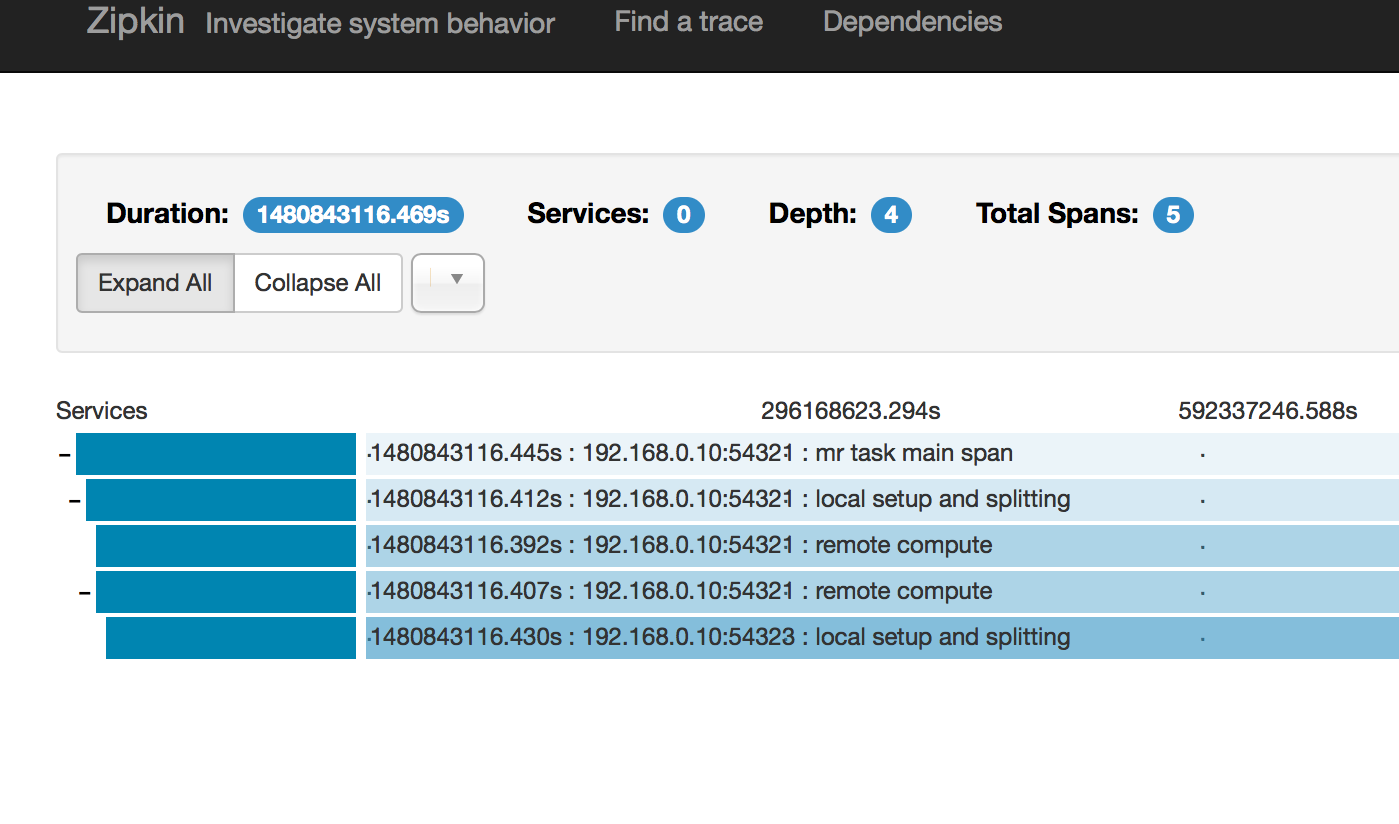
\includegraphics[scale=0.5]{zipkin_ui_example.png}
	\caption{Example of Zipkin UI}
	\label{fig:zipkin_ui}
\end{figure}

Each span in the UI is clickable and all the additional information can bee seen at that level. In this thesis the stack trace are also collected at each span for monitoring purposes. Example of such information screen can be seen on the figure \ref{fig:zipkin_ui_detail}.
\begin{figure}
	\centering
	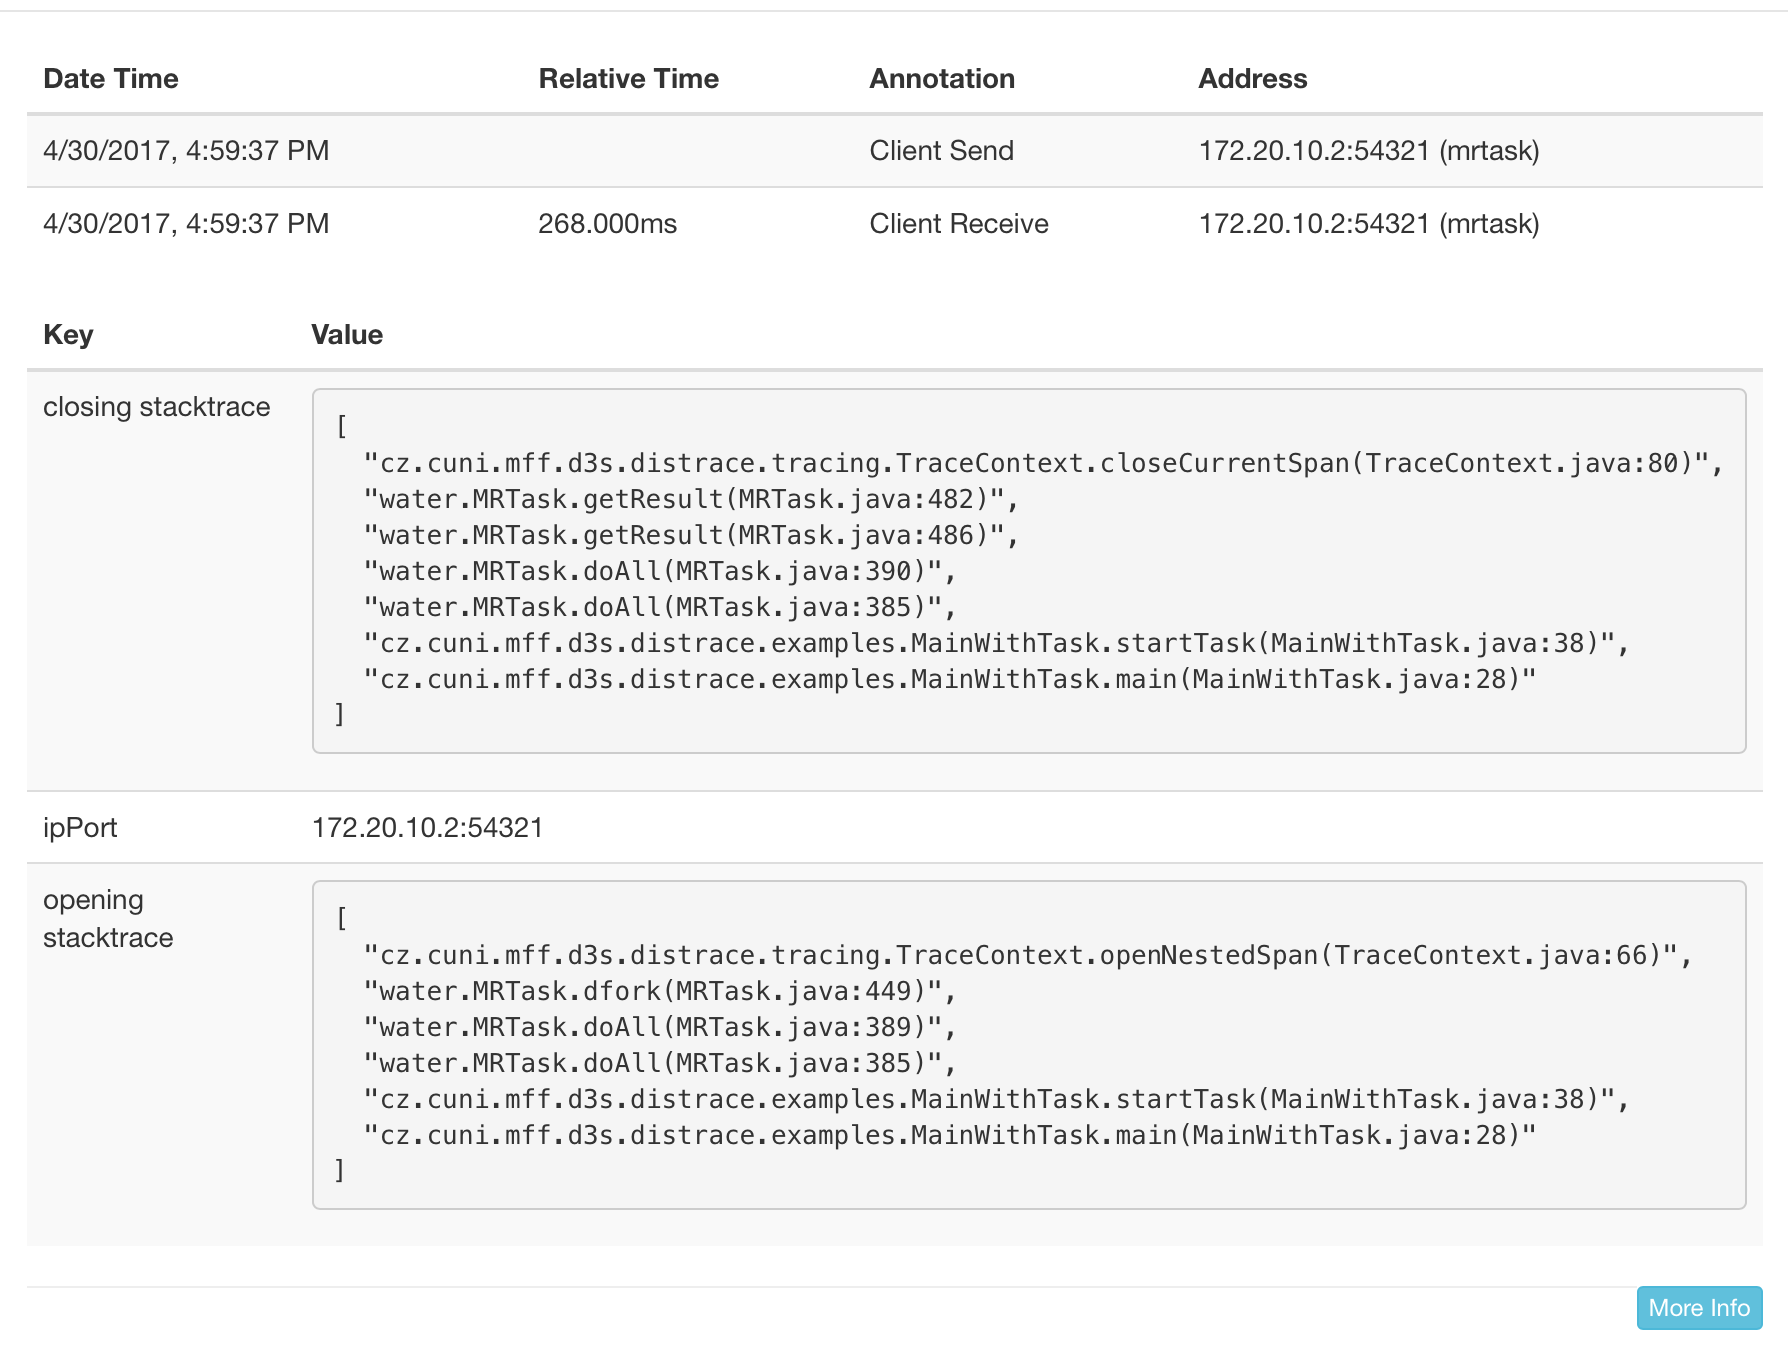
\includegraphics[scale=0.4]{zipkin_ui_detail.png}
	\caption{Example of the detail span information.}
	\label{fig:zipkin_ui_detail}
\end{figure}
\subsection{Zipkin Data Model}
Zipkin requires data to be sent in JSON format. Requests to UI are sent as JSON arrays where the array elements are the spans. Zipkin understands the following fields of Span object:
\begin{itemize}
	\item \textbf{traceId} - unique id representing the complete trace. It can be either 128 or 64 bit long.
	\item \textbf{name} - human readable span name
	\item \textbf{id} - id of this span. At the current implementation, Zipkin UI supports span ids only to be 64-bit long.
	\item \textbf{parentId} - parent id of the current span.
	\item \textbf{timestamp} - the time when the span was created.
	\item \textbf{duration} - the duration of the span. It is the duration between the span creation and span closing.
	\item \textbf{annotations} - array containing standard Zipkin annotations. These annotations can be handled by user interface in specific way since the user interface understands the meaning of the content. The documentation specifies the following annotations:
	\begin{itemize}
		\item \textbf{cr} : timestamp of client receiving the span
		\item \textbf{cs} : timestamp of client sending the span
		\item \textbf{sr} : timestamp of server receiving the span
		\item \textbf{ss} : timestamp of server receiving the span
		\item \textbf{ca} : client address
		\item \textbf{sa} : server address
	\end{itemize}
	\item \textbf{binaryAnnotations} - array of custom annotations. For example collected stack traces are sent as a binary annotation.
\end{itemize}

Except the \textit{annotations} and \textit{binaryAnnotations} fields, the fields are of simple string or number type. Annotations are objects with the three fields - annotation value, annotation name and the endpoint. Endpoint is another object specifying the address and port at the code where the span or particular annotation was recorded. Endpoints can also specify service name which may be used to search for particular spans.

Full example of data sent to Zipkin can be:
\begin{lstlisting}[emph={traceId, name, id, timestamp, duration, annotations, value, endpoint, serviceName, ipv4, port, binnaryAnnotations, key},emphstyle={\textbf}]
[
 {
    "traceId": "123456789abcdef",
    "name": "query",
    "id": "abcd1",
    "timestamp": 1458702548467000,
    "duration": 100743,
    "annotations": [
      {
        "timestamp": 1458702548467000,
        "value": "sr"
        "endpoint": {
          "serviceName": "example",
          "ipv4": "192.168.1.2",
          "port": 9411
        },
      }
    ],
    "binaryAnnotations": [
      {
        "key": "bytes_sent",
        "value": "1783"
        "endpoint": {
          "serviceName": "example",
          "ipv4": "192.168.1.2",
          "port": 9411
        },
      }
    ]
 }
]
\end{lstlisting}



\chapter{Implementation Details}
\label{chap:implementation}
This chapter explains several technical implementation details. The first section describes span exporters and API of Trace Context. The following section focuses on implementation details of the native agent and the last section focuses on the implementation details of the instrumentation server.

\section{Span and Trace Trees}
This section explains two implementation specific areas related to spans and trace trees. It describes span exporters in more detail and gives an overview of the Trace Context API. 
\subsection{Span Exporters}
\label{imp:exporter}
Implementation of span exporters have to extend from the abstract ancestor defining common methods for each span exporter. Also, in order to be able to use the exporter automatically in the code, it has to have a constructor with single \texttt{String} argument accepting exporter arguments. The arguments format is defined in the case of default span exporters, however the developer may use any format in case of custom span exporters. \texttt{SpanExporter} abstract class is the common ancestor for each exporter and has two abstract methods:
\begin{itemize}
	\item \texttt{export}. This method is used for exporting the span. Custom span exporters implementation may save the data on local disk or send over network. The destination is not limited by the code. Internally, the \texttt{export} method is called asynchronously in separated threads to allow asynchronous span exporting, which can lead to a performance benefit.
	\item \texttt{parseAndSetArgs}. The native agent has configuration property, which the user can use to configure arguments for the span exporter. Each span exporter is responsible for parsing its own arguments.
\end{itemize}

As mentioned in the Section \ref{design:exporter}, the Distrace tool provides two default implementations of span exporters:
\begin{itemize}
	\item  \texttt{DirectZipkinExporter} -  This span exporter sends the collected span asynchronously to the user interface right away without storing the data on disk to be collected by any data collection agent. In this case, the functionality of the span exporter and the data collector are handled by this single exporter.
	This span exporter should be used only for demonstration purposes, since it could overload the user interface or network when processing high number of spans, because the Zipkin user interface is not prepared to handle and store large amount of data in the memory. However, this is a default span exporter at this moment.
	
	This exporter accepts a single argument, which is the IP address and port of the Zipkin user interface. The Figure \ref{fig:zipkin_span_exporter} shows, how the Zipkin span exporter is used.
	
	\begin{figure}
		\centering
		
\includegraphics[scale=0.6]{zipkin_span_exporter.png}
		\caption{Using the Zipkin span exporter to export spans directly to Zipkin user interface without the data collection agent.}
		\label{fig:zipkin_span_exporter}
	\end{figure}
	\item  \texttt{JSONDiskExporter} - The second available span exporter saves the collected spans asynchronously on disk in the format known to the Zipkin user interface. The exported spans may be collected in the future by a custom data collection agent and for example, sent to the user interface or database. Together with some well-known data collection agent, this is a preferred way of transferring spans from the application to the Zipkin user interface in the production. This exporter accepts single argument, which is a destination directory for exported spans. The Figure \ref{fig:disk_span_exporter} shows how JSON disk span exporter is used.
	\begin{figure}
		\centering
		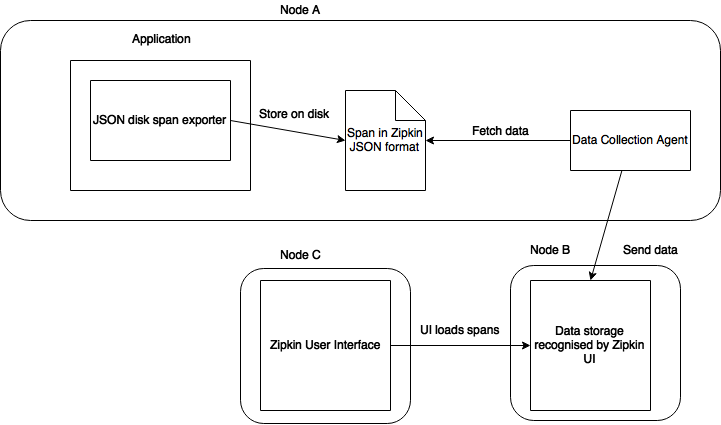
\includegraphics[scale=0.5]{disk_span_exporter.png}
		\caption{Using the JSON disk exporter together with the data collection agent together with the Zipkin user interface .}
		\label{fig:disk_span_exporter}
	\end{figure}
\end{itemize}
Additionally, the Figure \ref{fig:custom_span_exporter} shows how a custom span exporter may be used.

\begin{figure}
	\centering
	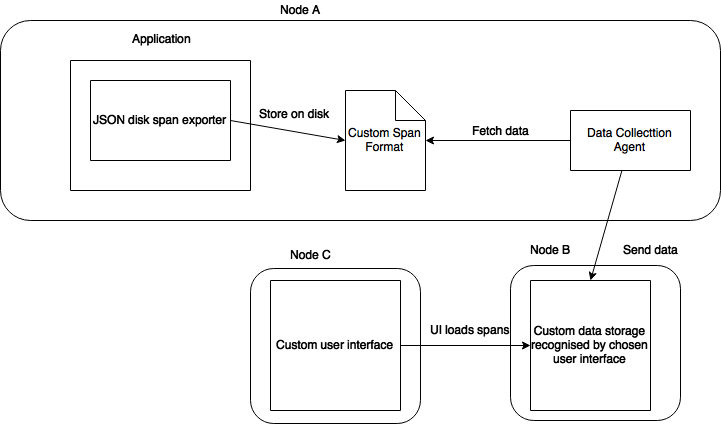
\includegraphics[scale=0.5]{custom_span_exporter.png}
	\caption{Using custom span exporter together with the data collection agent and custom user interface.}
	\label{fig:custom_span_exporter}
\end{figure}

In order to give the developer the flexibility to add new exporters without changing the internals, the custom service loader is used and the span exporters have to be registered in the META-INF directory of the extended instrumentation server JAR file. This ensures that the service loader can find all implementations of the \texttt{SpanExporter} abstract class. The reason why the classes need to be discoverable by the service loader is explained in the Section \ref{desing:native_initialization}.

To make the developer life easier, the \textbf{AutoService} library\footnote{The AutoService library is available at \url{https://github.com/google}.} may used when extending the core server library. Instead of manually registering implementations of custom span exporters into META-INF directory, they can be annotated in the code using the \texttt{AutoService} annotation. This annotation takes a single argument specifying the abstract parent, in this case \texttt{SpanExporter}. The library takes care of registering the classes automatically in the desired folder in correct format so the human error is minimized.

\subsection{Trace Context API}
\label{imp:trace_context_api}
The following methods can be used for obtaining and attaching the trace context:
\begin{itemize}
	\item \texttt{static create()} - creates a new trace context.
	\item \texttt{static getFromObject(holder)} - gets the existing trace context from the holder object.
	\item \texttt{static getFromThread(thread)} - gets the existing trace context from the specified thread.
	\item \texttt{static getFromCurrentThread()} -  gets the existing trace context from the current thread.
	\item \texttt{attachOnObject(holder)} - attaches the trace context to the holder object.
	\item \texttt{attachOnThread(thread)} - attaches the trace context to the specified \newline thread.
	\item \texttt{attachOnCurrentThread()} - attaches the trace context to the current \newline thread.
	\item \texttt{deepCopy} - creates a deep copy of the trace context. It is usually used in cases where child spans are processes in parallel by multiple threads. In this case, the copy of trace context with the same id is shared among all these threads, but they operate on very own objects. This is done in order to allow monitoring of parallel spans within a single trace without having to face race conditions on a single trace context object.
\end{itemize}

The methods above can also be chained and, for example, a trace context can be obtained from the holder object, deep copy created and the newly created copy attached to a new holder object.


\section{Native Agent}
This section covers specific parts of the native agent in more detail. It starts with explanation of considered approaches for instrumentation during the development. The problem of instrumentation server requiring the dependencies for each instrumented class is explained together with the problem of instrumenting the classes with cyclic dependencies. The final solution is explain as well. Further, the instrumentation API, which is used for communication with the server, is explained. Last section describes the byte code parsing.
\subsection{Instrumentation Details}
\label{imp:native:inst}
The native agent does not perform the instrumentation, but asks the server to carry out the transformation. The agent obtains the original bytecode for the class, sends the bytecode to the instrumentation server, waits for the transformed bytecode and lastly, applies the instrumented bytecode.

The instrumentation server requires all dependencies to be available for the the class currently being instrumented. This means that all other classes referenced inside the class file need to be available on the instrumentation server. This includes:
\begin{itemize}
	\item Argument types of all methods.
	\item Return type of all methods.
	\item Type of all fields.
	\item Type of a super class.
	\item Type of implemented interfaces.
\end{itemize}
The dependencies have to be loaded also for the referenced types. To achieve this, we tried two solutions, but only the second solution shown to be feasible.

\subsubsection{Unsuccessful Solution}
The first and unsuccessful solution was based on the fact that several \texttt{Class File load Hook} callbacks may be executed multiple times in different threads. When the application loads a class, the \texttt{Class File load Hook} event is triggered and bytecode ot this class is made available. In this method, the new \texttt{Class File load Hook} event was artificially enforced via the \texttt{RetransformClasses} JVMTI method. This method accepts array of classes for which the hook should be re-thrown. In order to continue with the instrumentation of the original class, all dependent classes have to be instrumented first. However, the classes with cyclic dependencies are not supported in this approach In order to instrumented a class with some cyclic references, all dependencies have to be instrumented first, which is also the class itself.

This solution faced also a different problem. Since the number of dependencies can be significant, the problem of too many threads being opened at a single time has also appeared. 

\subsubsection{Chosen Solution}
The second and currently used solution is based on the fact that Java class files may be accessed as a resource using the class loader, which is loading the class. The class file can be accessed using the \texttt{getResourceAsStream} method. Disadvantage of this solution is that developers may override this method in their applications and not provide access to the class files. This is a limitation of the thesis. However, when a such event happens, the instrumentation does not end with the exception, but the attempt to load the class using a different class loader created artificially is done. 

In this solution, the instrumentation server is first asked whether the class currently being loaded should be instrumented. If the class is marked for instrumentation, its bytecode is sent to the instrumentation server\footnote{This step is done only in case if the bytecode for the class is not already available}. Then, all references are scanned in the class file. For this, we need to parse the raw JVM bytecode. More details about this process is explained in the Section \ref{imp:parsing}. Loading of dependent classes is recursively called for each references class until the class does not have any other dependencies, or if all the dependencies are already uploaded on the instrumentation server. Once all dependencies for the class have been sent to the server, the instrumentation process is started and the agent waits for the transformed bytecode. 

\subsubsection{Initializers and Interceptors}
The instrumentation library used at the server (Byte Buddy) is using so called \texttt{Initializer} class to set up special interceptor field in the instrumented classes. It is a static field, which references the instance of the class interceptor. An interceptor is a class, which defines the instrumentation code. This interceptor field is automatically set by Byte Buddy framework using the corresponding initializers in most use-case of this library. However, in case of the Distrace tool, the instrumentation is performed in different JVM then where the code is actually running and Byte Buddy can't handle this case automatically. Therefore, setting of the interceptor field has to be handled explicitly.

In order to set this field by corresponding initializer, both the initializer class and interceptor class need to be available on the agent. The instrumentation server sends the initializer class together with the instance of interceptor during the instrumentation of the class. Upon receiving, the agent registers the interceptor and initializers with the instrumented class for later to be applied. The interceptor field is static and can be set up only when the class is used for the first time. Therefore, the initializers are loaded during \texttt{Class Prepare} event triggered by the JVM with the application and set up the interceptor field of the class. This event is triggered when the class is prepared, but no code has been execute so far. 

This is not required in case the Advice API is used for the instrumentation. More information about the Advice API is in the Section \ref{back:code_transform}.

\subsection{Auxiliary Classes}
Auxiliary classes are created at run-time during the instrumentation of a class by Byte Buddy framework. For example, proxy to a super class or proxy classes to fields accessed from the instrumented code are generated automatically as auxiliary classes. Any instrumented class using this pro requires these classes to be available at run-time on the JVM with the application. Therefore, the native agent asks the server for bytecode of the auxiliary class associated to with the currently instrumented class. After receiving, the native agent saves the bytecode as a Java class file on disk and makes the class available to the application by adding the class on the application's classpath.

\subsection{Instrumentation API}
The \texttt{Instrumentation API} provides several methods used internally to communicate with the instrumentation server. It defines low-level methods for sending data in form of byte arrays or strings and the corresponding methods for receiving the data. Several more complex methods are built on top of these basic ones to make the communication easier. The most important methods are in the API are:
\begin{itemize}
	\item \texttt{sendClassData} - sends bytecode to the instrumentation server.
	\item \texttt{isClassOnInstrumentor} - checks, whether the bytecode for a given class is already available on the instrumentation server.
	\item \texttt{instrument} - triggers the instrumentation and returns the instrumented bytecode.
	\item \texttt{loadInitializersFor} - loads initializers for a specific class.
	\item \texttt{loadDependencies} - loads all dependent classes and sends them to the instrumentation server.  A dependent class is uploaded only in case it's not already available on the instrumentation server.
	\item \texttt{shouldContinue} - checks if the class on its input is marked for the instrumentation.
	\item \texttt{loadPrepClasses} - loads all classes, which are required by the monitoring tool to be available at run-time on the JVM with the application. These are for example \texttt{TraceContext} and \texttt{Span} classes.
\end{itemize}

\subsection{Byte Code Parsing}
\label{imp:parsing}
Byte code parsing is necessary feature of the Distrace tool and is required for discovering the list of all dependent classes of a class currently being loaded. No sufficient C++ implementation has been found and therefore, a custom parsing module has been implemented. Byte code parsing module in the Distrace tool is inspired by the Apache Commons BCEL library\footnote{More information about this library can be found at \url{https://commons.apache.org/proper/commons-bcel/}.} written in Java. We created very simplified C++ equivalent of this library with features required for our needs.

The main entry point for parsing is the \texttt{ClassParser} class, which contains \texttt{parse} method accepting the bytecode of a class to be parsed. The \texttt{ClassParser} class also defines several accessors for the parsed information. For example, we can get name of the super class name, list of all implemented interfaces, list of all methods or list of all defined fields and their types.

The bytecode structure consists of several parts:
\begin{itemize}
	\item \textbf{Magic id} - Magic id is the first integer stored in each bytecode and is always set to 0xCAFEBABE hexadecimal number.
	\item \textbf{Version} - Version consist of two numbers of \texttt{short} type. The first short represents minor Java version and the second major Java version.
	\item \textbf{Constant pool} - Constant pool is a table, which contains mapping from id, representing a Java type, to the fully qualified type name. Id can represent interface names, field names and also other important constants.
	\item \textbf{Class Info} - Class Info contains the information whether the currently parsed bytecode represents a class or an interface. It also contains name of this class and name of the parent class.
	\item \textbf{Interfaces} - This part of bytecode contains the number of interfaces this class implements. This number is followed by id of type \texttt{short} for each interface. The fully qualified name of an interface can be looked up using the class pool.
	\item \textbf{Fields}. This part of the bytecode contains the number of fields this class defines together with some additional information for each defined field. The fully qualified type of a field can be looked up using the class pool.
	\item \textbf{Methods}. This part contains the number of defined methods in the bytecode together with some additional information for each method such as the number of arguments. The fully qualified types of return value and arguments of the method can be looked up using the class pool.
\end{itemize}
More information about the class file structure can be found at the official Java documentation\footnote{The documentation of the class loading process is available at \url{https://docs.oracle.com/javase/specs/jvms/se7/html/jvms-4.html}.}.
Each section of a class file is parsed separately. \texttt{ByteReader} class is used as a reader of the raw bytecode and contains several methods for reading different types of data from the bytecode array. 

Parsing the magic id and both, minor and major versions, is straightforward as they are just numbers and can be read using the \texttt{ByteReader} class directly. Parsing of the constant pool is more complex. For each entry in the constant pool a constant representing the entry is read. Each constant represent a specific object. For example a constant can represent a class, string, type of a field or return value and arguments of a method. Once the constant pool is parsed, it can be queried for the specific symbols using their id. Class name, super class name, interfaces, fields and methods are read from the constant pool using their ids.

\section{Instrumentation Server}
This section describes several technical parts of the instrumentation server. The details of the instrumentation itself are provided first, followed by an overview of the optimizations the server does to speed up the communication with the native agent. The next sections describes how trace context is injected to instrumented classes and how native methods at Java are bound to their implementations on the native agent side. The last section describes how JSON objects, which represent spans, are generated.

\subsection{Instrumentation Details}
\label{impl:server:instr}
The classes to be instrumented are marked using the \texttt{MainAgentBuilder} and \texttt{BaseAgentBuilder} classes.
The instrumentation server expects the instance of \texttt{MainAgentBuilder} on the input of its \texttt{start} method. This builder is the abstract class containing single abstract method \texttt{createAgent(BaseAgentBuilder builder, String pathToHelperClasses)}, where the builder is a wrapper \linebreak around the Byte Buddy \texttt{AgentBuilder} class, which is used to define the class transformers.

The developer extending the core instrumentation server needs to implement this method and specify on which classes and on which methods the instrumentation should happen. Since Byte Buddy is used for writing transformers and interceptors, more information about Byte Buddy library is located in the Section \ref{sec:byte_buddy}. In short, transformers are used to identify the class to be instrumented. They consist of advice or interceptors identifying the particular methods to be instrumented on the given class. The advice and interceptors also contain the code to be injected to the instrumented methods. The server provides several helper methods for creating the transformers and interceptors, which are less verbose then the standard Byte Buddy approaches.

Each interceptor has to implement the \texttt{Interceptor} interface. This is required so the server can discover all interceptor implementations at run-time without the need of changing the internals of the server. Each implementation of the interceptor needs to register itself in the META-INF directory of the generated JAR file in the same way as the span exporters mentioned in the Section \ref{imp:exporter}. Custom service loader is then used to locate all classes implementing the \texttt{Interceptor} interface. The interceptors need to be discovered since the instrumented classes depend on the interceptors and require them at run-time. Therefore, the instrumentation server have to send them to the native agent to make them available to the monitored application.

The advice may be used without any special annotations since Byte Buddy in-lines the code defined by the advice into the original code. Therefore, there is no need to transfer the advice implementations to the monitored application.

Even though Byte Buddy takes care of the internals of the instrumentation, the \texttt{BaseAgentBuilder} class is internally properly configured so the instrumentation is defined exactly as desired. This class implements four Byte Buddy listeners used reporting about the instrumentation progress. These listeners allow us to react on the process of the instrumentation. The listeners are:
\begin{itemize}
	\item \texttt{onTransformation} listener is called immediately before the class is instrumented. Implementation of the listener in the Distrace tool also sends to the agent all auxiliary classes required by the instrumented class and the initializers used for setting the static interceptor field on the instrumented class.
	\item \texttt{onIgnored} listener is called when the class is not marked for instrumentation. The class is not instrumented if the developer does not define any transformer for the specified class.
	\item \texttt{onError} listener is called when some exception occurred during the instrumentation.
	\item \texttt{onComplete} listener is called when instrumentation sucessu completed. It is called after both of \texttt{onTransformation} and \texttt{onIgnored} listeners.
\end{itemize}

Byte buddy requires all dependent classes for the instrumented class to be available. They are needed because the instrumentation framework needs to know signature of all methods so it can correctly identify the methods to be instrumented. The dependencies are all classes referenced in the class file such as type of the method return value and arguments, super class and implemented interfaces. 

By default, Byte Buddy library attempts to find these dependencies using  \texttt{LocationStrategy} and \texttt{PoolStrategy} classes. The first class is used to tell Byte Buddy where to look for the raw bytecode of dependent classes. By default, the classes are loaded by the context class loader, but since the classes to be instrumented are received over the network, custom \texttt{InstrumentorClassloader} class loader is used to handle the class loading. It is a simple class loader which loads the class data from the agent and caches them. When there is a request for instrumentation, instead of looking into the class files, this class loader loads the bytecode from the cache and passes it to the Byte Buddy.

However, Byte Buddy internal API does not work directly with raw bytecode. It uses classes \texttt{TypeDescription} and \texttt{PoolStrategy}. The first class has a constructor accepting the \texttt{Class} class. The  instance of this class contains metadata for the class passed to the constructor, such as the signature of all methods and fields, list of all interfaces or for example list of constructors. The second class is used for caching the type descriptions so they are not created every time the class is accessed. 

In overall, class lookup is done in the following two steps:
\begin{enumerate}
	\item Check whether type description for the class is available. If yes, load the type description from the cache.
	\item If the type description is not available, load the class using the \linebreak \texttt{InstrumentorClassloader}, create type description for the class and put it in the cache.
\end{enumerate}

\subsection{Optimizations}
The instrumentation server performs several optimizations to speed the communication with the native agent. The first optimization is caching of the classes sent to the instrumentation server from the native agent and also caching of already instrumented classes. This behavior is useful in cases where the native agents are sharing the instrumentation server. When a class is received from any agent, it is cached and the rest of the agents don't need to send the original class again when they request the instrumentation from the server. The server also performs the instrumentation only once and caches the instrumented classes. When any agent queries the server to instrument already instrumented class, the server can send the class immediately from the cache.

The second way how the communication can be optimized is influenced by the user. The user may compile the extended instrumentation server with the application classes or add these classes on the classpath of the server. When a native agent asks the server for instrumentation of a class, the server first check if it can load the class locally and avoid transferring the bytecode from the native agent. 


\subsection{Span Injection}
This short section explains how span and trace details are internally attached to the instrumented classes. The trace information is attached to the class by adding a new synthetic field with name \texttt{\_\_\_\_traceContext}. This trace context represents the current trace and is used in the code to obtain reference to a current trace context and also current span. This new field is created using the Byte Buddy instrumentation builder with the \texttt{defineField} method.


\subsection{Binding the Native Methods}
This section explains how methods implemented on the native agent can  be used in the classes defined on the instrumentation server. Some classes created at the instrumentation server, such as \textbf{SpanExporter} class, have to use data from the native agent. This is achieved by creating a helper method at the agent side, which returns the required data, and by creating corresponding native method on the Java side. When a class, which defines these native methods, is sent to the native agent and used for the first time, the native method in Java is bound to the implementation in C++. The methods are bound together inside the callback for the \texttt{Prepare} event. This ensures that we can define native methods in Java and bind them with their implementations on the separated machine, in this case the machine with the native agent. Also, this can have performance benefits, since these methods are written as native methods.

For example, this technique is used for accessing the span exporter type inside the \texttt{SpanExporter} abstract class. This class is defined at the instrumentation server, however the exporter type is passed as an argument to the native agent. This class contains the native method named \texttt{getSpanExporterType}, which returns the span exporter type. The \texttt{SpanExporter} class is sent to the native agent during the agent initialization and when it's used for the first time, the \texttt{getSpanExporterType} method is bound to the corresponding C++ implementation, which provides value of this argument.

\subsection{JSON Generation}
\label{json_gen}

The collected data inside spans are internally stored as instances of \texttt{JSONValue} class representing any JSON value. JSON format is chosen since default Zipkin user interface expects spans in this format. JSON is a lightweight format for exchanging data with the syntax based on Javascript object notation.

The JSON handling is inspired by the minimal-json library\footnote{The library is available at \url{https://github.com/ralfstx/minimal-json}.}. The simplified custom implementation was created which provides features required by the Distrace tool. Also the number of dependencies required to build is tool is lowered since this code is part of the Distrace sources.

This JSON support is designed via several classes:
\begin{enumerate}
	\item \textbf{JSONValue} - The abstract ancestor for all JSON types. This type defines common methods to all implementation.
	\item \textbf{JSONString} - A class representing string types.
	\item \textbf{JSONNumber} - A class representing numeric types.
	\item \textbf{JSONLiteral} - A class representing the literals \textbf{null}, \textbf{true} and \textbf{false}.
	\item \textbf{JSONArray} - A class representing the JSON arrays. It has support for adding new elements into the array.
	\item \textbf{JSONObject} - A class representing the JSON objects. It has support for adding a new items into the object.
\end{enumerate}

Each \textbf{JSONValue} can be exported as string where the printing is driven by the \texttt{JSONStringBuilder} class. This class is also responsible for escaping the characters according to JSON standards. The default printer exports the data without any formatting into a single text line, however \texttt{JSONPrettyStringBuilder} exports the data in more human-readable format. The second printer is usually used for the debugging purposes and the first one is used for exporting spans in real scenario as the size of the data is smaller in this case.



\chapter{Realistic Case Study}
\label{chap:big_example}
This chapter demonstrates how the Distrace tool can be used on a bigger example and also serves as the user manual for creating custom monitoring applications. We will go through all the steps from creating the application up to running the application and accessing the observed results.

This example is based on the H\textsubscript{2}O\footnote{More information about H\textsubscript{2}O can be found at \url{https://www.h2o.ai} and \url{https://github.com/h2oai}.} open-source fast scalable machine learning platform. This platform supports various methods for building machine learning models, methods such as deep learning, gradient boosting or random forests. The core of the H\textsubscript{2}O platform is written in Java and clients for different languages exist as well. Internally, H\textsubscript{2}O is using map-reduce computation paradigm\footnote{Map-reduce is a programming model in distributed systems. The basic idea is to split tasks into smaller parts and perform the map operations. The intermediate results are then combined together using the reduce calls until the complete result has been assembled from all the sub-tasks.} to perform various tasks across the cluster.

The goal of this example is to monitor a subset of map-reduce tasks and see visualizations of the computation process. This can help reasoning about the performance of the platform and can discover unwanted delays in the computations. This chapter first describes relevant parts of the H\textsubscript{2}O platform in more details. In the following sections, we describe in steps how to extend the core instrumentation library for H\textsubscript{2}O purposes. Lastly, we show how this example can be started and how visual outputs can be interpreted. 
This full example is also available in the attached source code of the thesis in the Attachment 1. More examples are available and their complete list together with the instructions on how to run them are in the Attachment 2.

\section{H\textsubscript{2}O In More Details}
H\textsubscript{2}O is in-memory machine learning platform. The platform is distributed and the computations are performed in the cluster. All nodes in the cluster are equal and each of them can initialize the computation. Most computations are performed as map-reduce tasks. This section describes the internal format of data used in the H\textsubscript{2}O platform, how data are stored on the nodes and lastly, how the computations are performed in the cluster. 

\subsection{Data in H\textsubscript{2}O}
Data is stored in H\textsubscript{2}O in so-called \texttt{Frames}. A \texttt{Frame} is column based distributed data table with columns and rows. The \texttt{Frame} is designed in a way, that it can handle data too big to fit into a memory of a single machine. Each column is represented by the \texttt{Vec} class. This class represents a vector of data that is again distributed across the nodes in the cluster. Further, each vector is split into multiple \texttt{Chunks} and each chunk represents the part of the vector physically available on a single node. Therefore, chunks are units of parallelization and distribution.

Hence, it is possible for one node to contain multiple chunks from a single vector and therefore, the number of chunks in the vector does not represent the number of nodes on which the data is distributed. Typically, data imported to H\textsubscript{2}O is distributed via chunks equally among all the nodes in the cluster, but algorithm may also decide to distribute the data on just several nodes in the cluster. It is also possible to create the frame manually and specify on which nodes the chunks will be stored. Therefore, the frame may be distributed only on a portion of the cluster. Usually, when chunks are being created on some specific node, chunks of the same size for each column are created on that node. This means that each node storing the data usually have corresponding (neighbor) chunks for all the columns. This can be thought of as that each node storing some data has a subset of rows from the full table with all columns. The point of this paragraph is that the distribution of chunks controls the parallelization.

The Figure \ref{fig:h2o_frame} shows the structure of a frame with three columns, where each column is split into two chunks. It also shows how chunks may be distributed in the cluster of size three. We can also see in the figure that corresponding chunks for each vector have the same size and are stored on the same nodes. Also, it is important to mention that data in H\textsubscript{2}O is not replicated.

	\begin{figure}
		\centering
		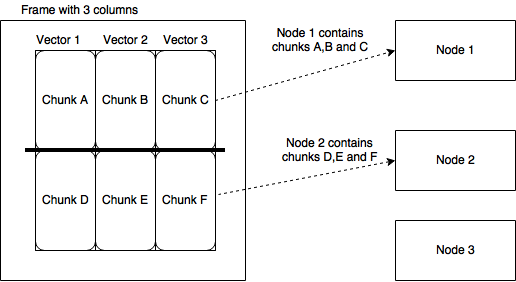
\includegraphics[scale=0.5]{h2o_frame.png}
		\caption{Structure of the H\textsubscript{2}O frame and its distribution in the cluster.}
		\label{fig:h2o_frame}
	\end{figure}

\subsection{Computation in H\textsubscript{2}O}
When the user tells H\textsubscript{2}O to create a deep learning model based on the data on the input, H2O sees this as a \textbf{Job}. Jobs are used for tracking long-lifetime user interactions and encapsulate the whole computation from the user point of view. The job encapsulates computation tasks of several map-reduce tasks. In H2O, the class \texttt{MRTask} is used as the core implementation of a map-reduce task\footnote{Different type of tasks exist in H\textsubscript{2}O, however only \texttt{MRTasks} are mentioned here since they are important to this example.}. The map-reduce task is always bound to some H\textsubscript{2}O frame on which the computation needs to be performed. This class is used to encapsulate the task, partition it to smaller tasks and run remote computations among the whole cluster. 

Each task contains the information about on which H\textsubscript{2}O nodes the task itself and its sub-tasks can be computed. When a task is split, this range is divided and each sub-task can be computed on the half of the nodes the parent tasks specifies. The task is executed on each H\textsubscript{2}O node which contains chunks required for this task. The \texttt{map} operations are called on each node, which contains locally available chunks for the frame this task is based on. The \texttt{reduce} calls are used to reduce the results from two sub-tasks into a new task combining results from the children.

In more details, the \texttt{MRTask} class extends from the \texttt{DTask} class. This class is a general class used in H\textsubscript{2}O to represent a task remotely executed. Further, the \texttt{DTask} class extends from the \texttt{H2OCountedCompleter} class. The last mentioned class is a simple wrapper around the Fork/Join (F/J) execution framework\footnote{More information about the Fork/Join framework can be found at the Java documentation available at \url{https://docs.oracle.com/javase/tutorial/essential/concurrency/forkjoin.html}.} allowing the platform to prioritize tasks. The Fork/Join framework is an implementation of Java \texttt{ExecutorService}, which helps with job parallelization on multiple processors. The Fork/Join framework executes tasks in separated threads and can move tasks between threads to ensure the highest possible performance. Each H\textsubscript{2}O \texttt{MRTask} is executed as \texttt{ForkJoinTask} inside this execution framework. A \texttt{ForkJoinTask} is a task wrapper, which is executed in a single thread. It is a light-weight wrapper and a large number of tasks may be served by a smaller number of actual threads.

The way how H\textsubscript{2}O perform computations from the high-level point of view can be seen in Figure \ref{fig:h2o_overview}. The task initiator receives the \texttt{MRTask} from the parent \texttt{Job} or from the user. It splits the task into two new sub-tasks and sends these tasks to up to two different nodes in the cluster. These nodes again split the task from the input and send the task to another selected nodes in the cluster. Each splitting decreases the number of nodes on which the task has to be sent. Once this number is equal to one, the node is marked as a leaf node and does not perform any other splitting and re-sending.

\begin{figure}
	\centering
	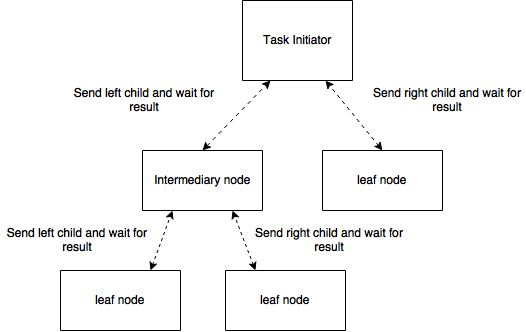
\includegraphics[scale=0.5]{h2o_overview.png}
	\caption{High-level overview of execution hierarchy.}
	\label{fig:h2o_overview}
\end{figure}

It is important to say that the \texttt{MRTask} is always distributed to all nodes in the cluster. This figure shows how it is ensured that each node participates in the computation, however, the computation step itself is still missing. Each node of the cluster, who receives a task, also submits the task for computation into the Fork/Join execution framework. This computation performs the mapping operation on all the chunks, which are available locally on the node executing this task, for the frame associated to the task. The \texttt{reduce} operation follows the \texttt{map} operation, however, we need to first ensure that the child tasks, from which we want to combine the results together, are already finished. This is ensured by child tasks signaling to the parent tasks when the work has been finished. Therefore, parent tasks are informed when they can start reducing the results. 

The computation on a single node is shown in the following pseudo-code:
\begin{lstlisting}[language=Java]
public void singleNodeComputation(){
  MRTask task = ... // task received from the parent or from the user
  MRTask left = split(task, start1, end1)
  MRTask right = split(task, start2, end2)
  remoteCompute(left)
  remoteCompute(right)
  H2O.submitTask(task) // submit this task into local F/J
  ..
  // task is taken from F/J for execution
  task.map(..)
  task.waitForComplete() // wait for the child tasks to finish
  task.reduce(left, right)
  notifyComplete(task) // notify the parent of completion
}
\end{lstlisting}
The split method accepts indices representing the nodes in the cluster on which this sub-task and further sub-sub-tasks may be executed.

The last missing piece of information is a description of what is done when the node has more chunks available for the frame associated with the task since each \texttt{map} operation is executed only per single chunk. In case the node has multiple chunks available for the frame, the node always locally submits two new tasks into the F/J framework, each having half of the chunks. This is recursively repeated until we have single chunk tasks, which are processed normally. These locally-split tasks inform their parents that they are done. This signalization goes up the tree until the original task is marked finished.

\subsection{Methods for Instrumentation}
For the purpose of this example, a special \texttt{MRTask} called \texttt{SumMRTask} has been created. This task just performs distributed sum of range of numbers. In order to be able to visualize the computation process of this task, the following \texttt{MRtask} methods were identified for the instrumentation:
\begin{itemize}
	\item \texttt{dfork} - this method is called at the initiator node and starts the computation of the whole task.
	\item \texttt{getResult} - this method is called at the initiator and blocks until the distributed computation finishes.
	\item \texttt{setupLocal0} - this method splits the task, creates sub-tasks for child nodes, sends the sub-tasks to the target child nodes and submits the local task.
	\item \texttt{map} - the map operation. This method needs to be implemented explicitly by the user. 
	\item \texttt{reduce2} - the reduce operation. This method needs to be implemented explicitly by the user. 
	\item \texttt{compute2} - this method controls the computation and internally calls the \texttt{map} implementation.
	\item \texttt{onComplete} - this method waits for the sub-tasks to finish and then calls the \texttt{reduce2} operation on them.
\end{itemize}

We are also interested in how long the remote computation lasts on child nodes. For this reason, we need to instrument the following two methods on the \texttt{RPC} class:
\begin{itemize}
	\item \texttt{call} - this method is called when the remote computation has been submitted.
	\item \texttt{response} - this method is called when the remote computation has been finished and the child node is signaling that its work is done.
\end{itemize}

\section{Building the Core Server and Native Agent}
In order to be able to extend the core instrumentation library, we need to build it first. This won't be necessary once the core instrumentation server is published to some online repository of JAR packages\footnote{For example, Maven Central Repository.}. The native agent also needs to be built on the platform where H\textsubscript{2}O will be running. 

Please see the Attachment 3 for the information on how to build the project from sources or how to run this example from the prepared Docker machine. 

\section{Extending the Core Instrumentation Server}
In order to capture the relationships between tasks and their computations, we need to instrument the methods mentioned in the previous section. It is important to always find a good pair of methods, which open and close a single span. In the case of H\textsubscript{2}O, the following calls have been identified to form good spans. The pairs are ordered from the top level spans encapsulating the whole computation to the local spans encapsulating single mapping or reduce operations.

\begin{enumerate}
	\item \texttt{dfork} - \texttt{getResult}. This pair forms the main span, which encapsulates the complete computation of a single \texttt{MRTask}. This is possible since the \texttt{dfork} method is only called on the node where the computation starts and the same holds for the \texttt{getResult} method after the computation finished. The span is opened when the first method is entered and closed when the latter method is left.
		
	\item \texttt{setupLocal0} - \texttt{onCompletion}. This pair forms the span representing the complete computation on a single node. It encapsulates the local work as well as the waiting for the remote work to complete. This span is opened when the first method is entered and closed when the latter method is left. This span is well-defined since the \texttt{onCompletion} method is called for each task and represents that the work has been finished in all children tasks.
	
	\item \texttt{call} - \texttt{response}. This pair forms the span used to track only the remote computation. It encapsulates the remote computation and all following sub-tasks created by the remote task. This span is opened when the first method is entered and closed when the second method is left.
	
	\item \texttt{compute2} - \texttt{onCompletion}. This pair forms the span used to encapsulate the local computation on a local node. It encapsulates all the cases of local work. In the case of multiple chunks exist for the given local task on the same node, this method is recursively called on split tasks until we have tasks representing a single chunk. The calls are also recursively confirmed by the \texttt{onCompletion} call. In multi-chunk case, only one child task is submitted for the execution into F/J thread. The second task is executed immediately in the same thread. This way it is ensured that we can reuse the existing thread as much as possible. This span is opened when the first method is entered and closed when the latter method is left.
	
	\item \texttt{map} - \texttt{map}. This pair represents the single mapping operation. This span is entered when the \texttt{map} method is entered and closed when the \texttt{map} method is left. Therefore, this span lasts only for the duration of the \texttt{map} method call.
	
	\item \texttt{reduce2} - \texttt{reduce2}. This pair represents the single reduce operation. This span is entered when the \texttt{reduce2} method is entered and closed when the \texttt{reduce2} method is left. Therefore, this span lasts only for the duration of the \texttt{reduce2} method call.
\end{enumerate}

For all of the pairs above, the Advice API is used for the instrumentation because it's sufficient in our case to be able to capture just method enter and exit events. In case we would like to perform more complex instrumentation, we could use the Interceptors API, which is described in the Byte Buddy documentation and briefly also in Section \ref{sec:byte_buddy}.

Instrumenting these methods is a technical task and the code can be seen in the corresponding example available in the Attachment 1. The trace context information is always attached to the task transferred between the nodes. The trace context is initially created during the \texttt{dfork} method call since it's the main entry point of the computation. When instrumenting the \texttt{compute2} and \texttt{setupLocal0} methods, the deep copy of the trace context is attached to the transferred task because the closing \texttt{onComplete} method is usually called from a different thread and this ensures there are no collisions caused by accessing the same trace context from multiple threads.

Also, when instrumenting a few of the mentioned methods, we need to ensure that correct pairs of spans are created and closed. For this purpose, we use flags available on the \texttt{Span} class. Flags allow us to attach additional information to the trace context, which may be used when closing the span. This is, for example, useful in cases when a method is used to close several spans at the same time and we need to properly distinguish between the spans to close the correct one.

Once all the advice or interceptors are created for each of the mentioned methods above, we need to create the transformers. The transformer defines on which method from the code of the application which advice or interceptor is applied. For this purpose, Distrace provides several helper methods allowing us to create transformers in a very concise way. For example, the transformer for \texttt{RPC.class} defining the instrumentation of the \texttt{call} and \texttt{response} methods looks like:

\begin{lstlisting}[language=Java]
new BaseTransformer() {
  @Override
  public DynamicType.Builder<?> 	defineTransformation(
    DynamicType.Builder<?> builder) {

    // Method to instrument
    Method call = ReflectionUtils.getMethod(RPC.class, "call");

    // Apply the advice on the method
    return builder
        .visit(Advice.to(RPCAdvices.call.class).on(is(call)))
        .visit(Advice.to(RPCAdvices.response.class).on(named("response")));
    }
}
\end{lstlisting}
The \texttt{RPCAdvices.call} and \texttt{RPCAdvices.response} static classes are the advice, which define the instrumentation.

Once the transformers for each method to be instrumented are created, we need to associate the transformers with the classes from the application on which they should operate. We also need to create a main entry point of the extended instrumentation server. This is demonstrated on the following code snippet:

\begin{lstlisting}[language=Java]
public static void main(String args[]) {
  new Instrumentor().start(args, new MainAgentBuilder() {
    @Override
    public AgentBuilder createAgent(BaseAgentBuilder builder, 
                                      String pathToHelperClasses) {
	 		 
	 		 return builder
		 		.type(isSubTypeOf(MRTask.class))
				.transform(mrTaskTransformer)
				.type(is(RPC.class))
				.transform(rpcTransformer)
	         }
	  });
}			 
\end{lstlisting}
In this code, we associate classes containing the methods to be instrumented to the transformers handling the instrumentation of those methods. We are also starting the instrumentation server using the \texttt{start} method provided by the core instrumentation server with the \texttt{MainAgentBuilder} instance as the argument. This instance is later used as a dispatcher of the instrumentation of the whole application. Later, when starting the application with the native agent attached and configuring the agent, we need to explicitly specify the class, which is used as the main entry point of the extended instrumentation server. This is exactly the class containing the \texttt{main} method with the content above.

At this step, we need to build the extended instrumentation server. This server has two dependencies: the core instrumentation server and also the H\textsubscript{2}O application sources. The first dependency is obvious as we are using the API defined in the core server library. The second library is required since we are using several application classes when defining the instrumentation points. This may not be necessary when instrumenting different applications since we can identify a class to be instrumented, for example, by its name using the following element matcher \texttt{named("fully.qualified.class.name)} instead of \texttt{is(Example.class)}. However, the second option gives us more freedom when defining the instrumentation points and has also a performance benefit. In this case, the application classes are already located on the server and when they are requested to be instrumented, the  bytecode for each of these classes doesn't have to be sent from the native agent. 

After this step, we should have two artifacts - the native agent library built for our platform from the previous steps and also the extended instrumentation server JAR file from this step.
\section{Configuring and Running the Application}
For the purposes of this example, we start the cluster of three H\textsubscript{2}O nodes. Two nodes are the regular nodes and the last node contains the main method in which the \textbf{SumMRTask} is executed. This task is used to sum up a range of numbers in distributed manner.

An arbitrary H\textsubscript{2}O node can be started as: \newline \texttt{java -jar h2o.jar -name cluster\_name}.\newline When operating on the network with multi-cast communication enabled, multiple nodes started with the same cluster name automatically forms a single cluster.

If we want to start the application with the monitoring agent attached, we can use the \texttt{-agentlib} java option. Any H\textsubscript{2}O node can be started with the monitoring feature enabled by calling the following command: \newline
\texttt{java -agentpath:"\$NATIVE\_AGENT\_LIB\_PATH=\$AGENT\_ARGS" -jar h2o.jar  \newline -name cluster\_name}

The \texttt{\$NATIVE\_AGENT\_LIB\_PATH} variable needs to point to the location of the native agent library and \texttt{\$AGENT\_ARGS} shell variable may contain any arguments passed to the native agent. The arguments are in the format \texttt{key=value} and are separated by the semicolon. The complete list of available arguments is in the Attachment 4.

In the case of this example, we let the native agent start the instrumentation server locally for each node automatically. Therefore, the inter-process communication is used and we don't need to configure it explicitly. Only two arguments need to be specified - the path to the instrumentation server and the fully qualified name of the main entry class of the instrumentation server.

Therefore, the full command starting H\textsubscript{2}O with the monitoring agent enabled is: \newline
\texttt{java -agentpath:"/home/agent.so=instrumentor\_server\_jar=\newline/home/instrumentor.jar;instrumentor\_main\_class=main.entry.pint" \newline-jar h2o.jar -name cluster\_name}

In order to start the cluster of size three, we need to call this command three times. Twice with the regular H\textsubscript{2}O node and once with the H\textsubscript{2}O node containing the execution of the \texttt{SumMRTask}. It is also important to start the Zipkin user interface to which the results are published. The user interface server may be started as: \texttt{java -jar zipkin.jar}\footnote{Zipkin Jar file may be downloaded at \url{https://github.com/openzipkin/zipkin} or is available at the attached CD.}.
\section{The Results}
Once all three nodes have been started, the computation starts and the results based on our instrumentation are shown directly in the Zipkin user interface. By default, the user interface is available at port 9411.

We need to click on the \textit{Find Traces} button to show all traces, which satisfy our search conditions. We should see in the output a single trace and once we click on it, we should see a similar result to the one in Figure \ref{h2o_zipkin_output}. This figure shows just a portion of the whole trace but contains the important observed information.
	\begin{figure}
		\centering
		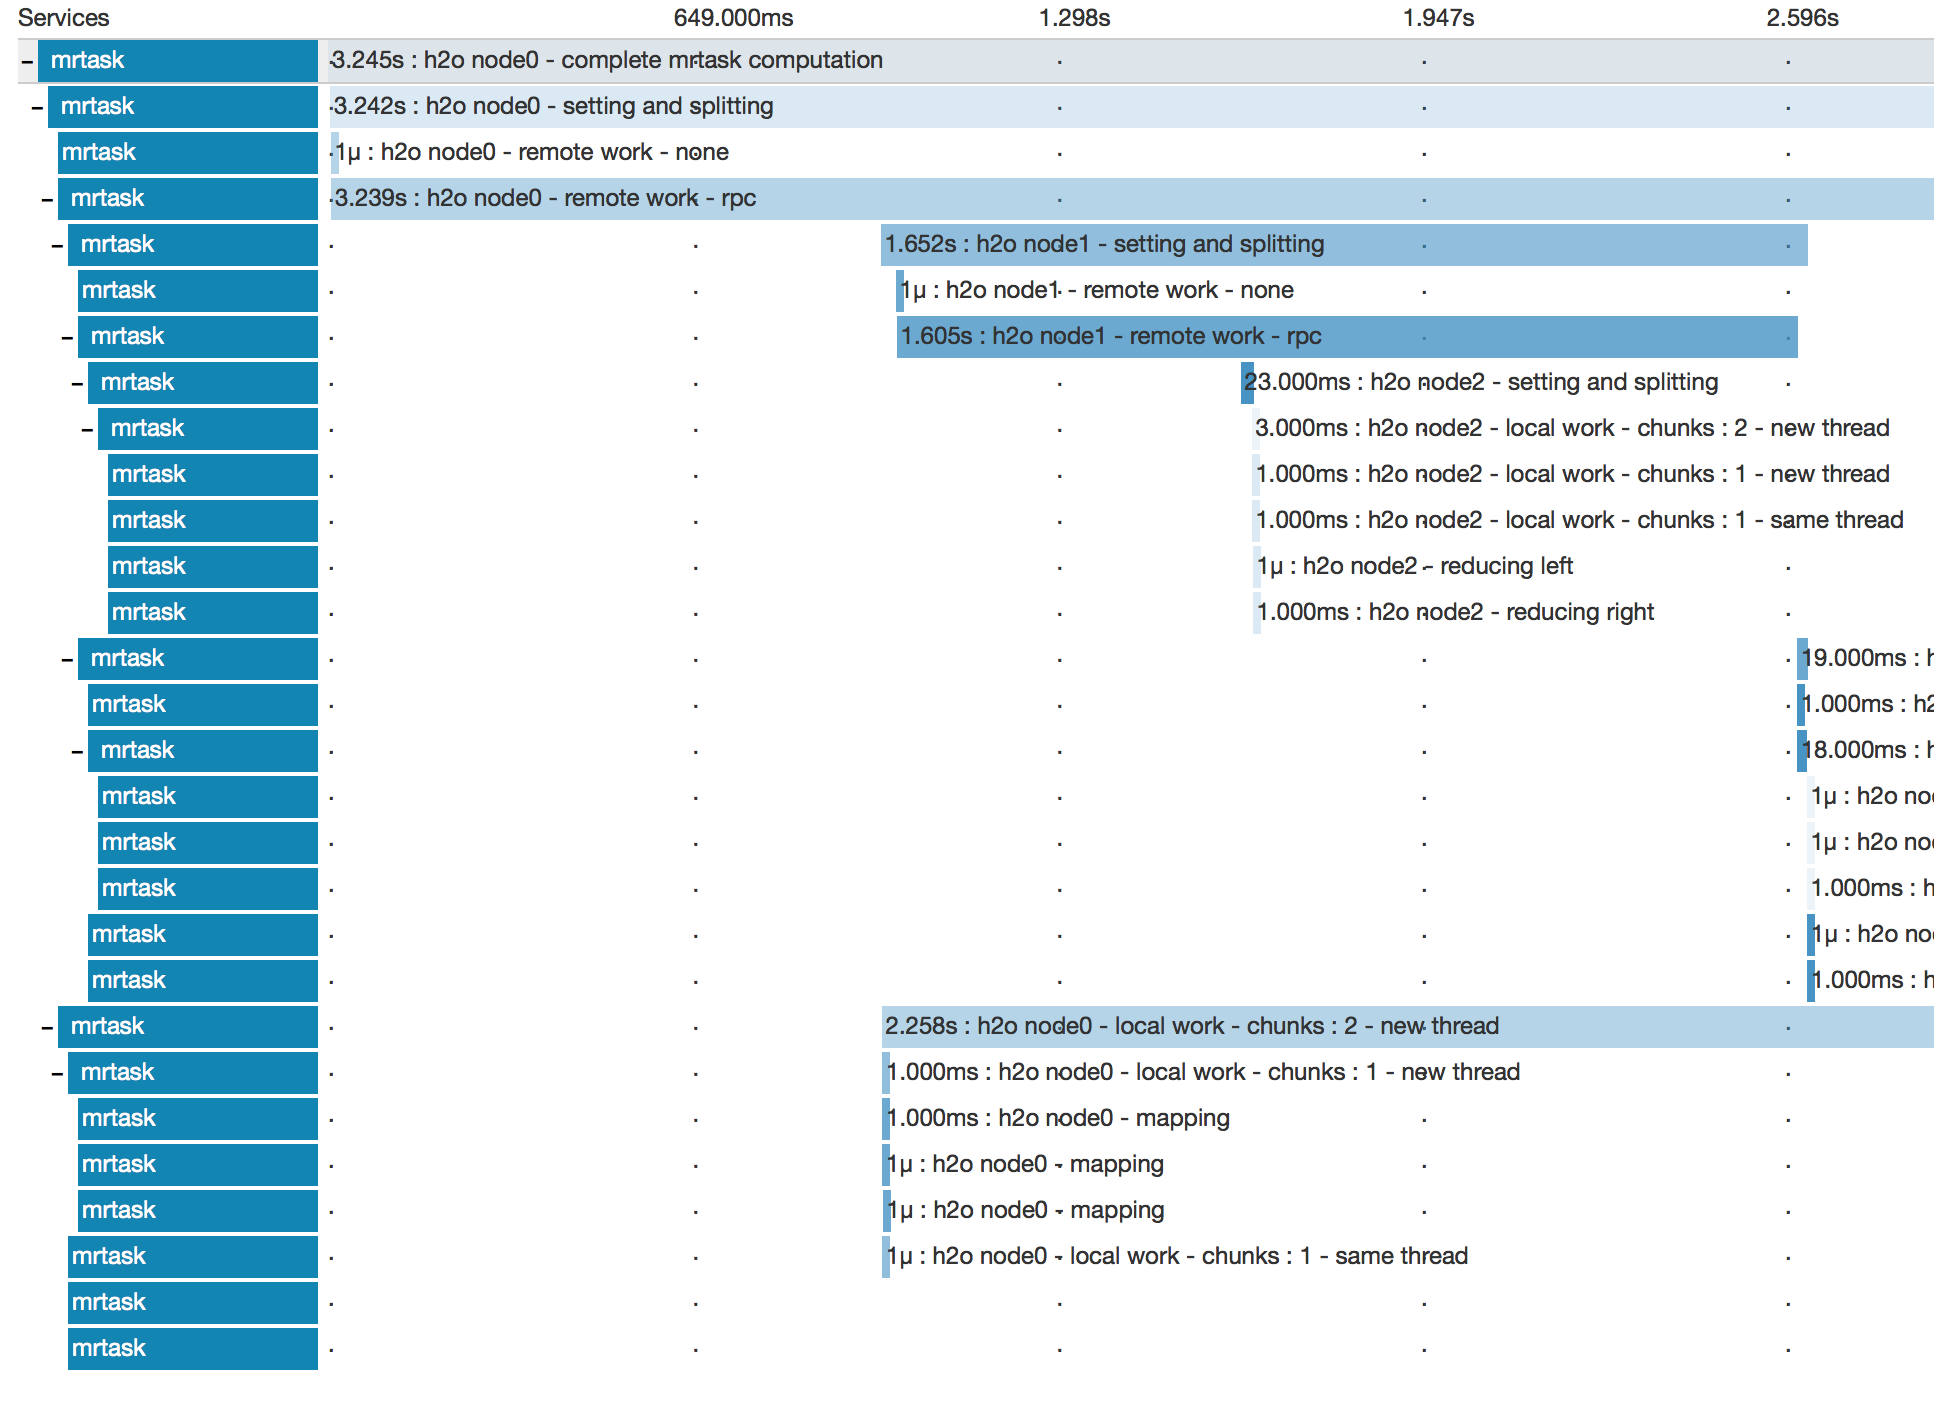
\includegraphics[scale=0.4]{h2o_zipkin_output.png}
		\caption{Example trace from the distributed computation on H\textsubscript{2}O platform.}
		\label{h2o_zipkin_output}
	\end{figure}

All the operations and their timing can be seen on the output and we can see how long each operation lasted and when it started. The spans are also organized hierarchically as they were created. We can see the main span encapsulating the whole computation, the spans for computation on each node and also spans encapsulation the remote computations. The local \texttt{map} and \texttt{reduce} calls are displayed as well. It is, for example, interesting to see how long it took the platform to perform the \texttt{reduce} operation after the \texttt{map} operation has been called.
\chapter{Evaluation}
\label{chap:evaluation}
\section{Known Limitations}
here mention limitations with the instrumentation


Appendix!
\section{Platform demonstration}
\subsection{Deployment Strategies}
\subsubsection{Instrumentor per Application Node}
\subsubsection{Instrumentor per Whole Cluster}
\subsubsection{Optimizing the Deployment}
\subsection{Basic Building Blocks}
\subsection{Basic Demonstration}
\subsection{Optimizing the Solution}

grafy
\chapter{Conclusion}
The main goals of this thesis were to create a monitoring tool for distributed Java applications with a small footprint on the monitored application and high-level application transparency and tool universality. It was also desired to ensure the usage and deployment of the final tool are simple. 

The instrumentation overhead can be still observed even though the classes are instrumented in a separated instrumentation machine, however, it is just a constant overhead based on the nature of the injected code to the original classes. The Distrace tool universality was achieved by implementing the native agent universal to all Java applications and by creating a core instrumentation server. This core server can be extended by developers and they can create application specific instrumentation tools. This also ensures that the final users of the monitored application does not need to know about the monitoring and can work with the application as usual. The developer has also the possibility to extend the monitoring platform by a custom user interface and can also specify a custom format for spans being exported from the application. This ensures that the Distrace tool may be integrated easily into already existing environments. The interface at the core instrumentation server is kept simple in order to make the usage straightforward also for developers.

Comparing to related Google Dapper, the Distrace tool introduced by this thesis is released as open-source and allows higher application transparency since the purpose of Google Dapper is to monitor only Google applications. Comparing to Zipkin, the user does not need to change the application sources in order to attach span and trace information. This ensures that the source code of the original application remains unchanged. The tool provided by this thesis does not aim to replace any of the mentioned tools, however, it tries to create a universal tool with keeping performance in mind and ensuring that the usage is a simple as possible for the end-user.


This Distrace tool is also planned to be extended in the future in the following areas:
\begin{itemize}
	\item \textbf{More Additional Span Exporters} \newline
	Currently, the Distrace tool provides two default span exporters and allows the user to extend the \texttt{SpanExporter} abstract class and implement custom ones. However, we would like to create more exporters in the future, which would be able to store spans into different storage types and also in different formats. At this moment, the output is in the JSON format understandable to the Zipkin user interface and the data are exported either to a disk or are send to the user interface right away. We could, for example, create a span exporter, which could export spans into a database, from which the arbitrary user interface could fetch the data.
	\item \textbf{Support for Flame Graphs} \newline
	The second future plan is to add support for flame graphs. The native agent could be used to capture the stack-traces of the running application and later, a flame graph representing the distributed computation could be created. For example, this integration would give us the ability to inspect the memory usage or performance cluster-vise using the flame graphs visualisations.
\end{itemize}



%%% Bibliography
%%% Bibliography (literature used as a source)
%%%
%%% We employ bibTeX to construct the bibliography. It processes
%%% citations in the text (e.g., the \cite{...} macro) and looks up
%%% relevant entries in the bibliography.bib file.
%%%
%%% The \bibliographystyle command selects, which style will be used
%%% for references from the text. The argument in curly brackets is
%%% the name of the corresponding style file (*.bst). Both styles
%%% mentioned in this template are included in LaTeX distributions.

\bibliographystyle{plainnat}    %% Author (year)
%\bibliographystyle{unsrt}     %% [number]

\renewcommand{\bibname}{Bibliography}

%%% Generate the bibliography. Beware that if you cited no works,
%%% the empty list will be omitted completely.

\bibliography{bibliography}

%%% If case you prefer to write the bibliography manually (without bibTeX),
%%% you can use the following. Please follow the ISO 690 standard and
%%% citation conventions of your field of research.

% \begin{thebibliography}{99}
%
% \bibitem{lamport94}
%   {\sc Lamport,} Leslie.
%   \emph{\LaTeX: A Document Preparation System}.
%   2nd edition.
%   Massachusetts: Addison Wesley, 1994.
%   ISBN 0-201-52983-1.
%
% \end{thebibliography}

%%% Figures used in the thesis (consider if this is needed)
\listoffigures

%%% Tables used in the thesis (consider if this is needed)
%%% In mathematical theses, it could be better to move the list of tables to the beginning of the thesis.
%\listoftables

%%% Abbreviations used in the thesis, if any, including their explanation
%%% In mathematical theses, it could be better to move the list of abbreviations to the beginning of the thesis.


%%% Attachments to the master thesis, if any. Each attachment must be
%%% referred to at least once from the text of the thesis. Attachments
%%% are numbered.
%%%
%%% The printed version should preferably contain attachments, which can be
%%% read (additional tables and charts, supplementary text, examples of
%%% program output, etc.). The electronic version is more suited for attachments
%%% which will likely be used in an electronic form rather than read (program
%%% source code, data files, interactive charts, etc.). Electronic attachments
%%% should be uploaded to SIS and optionally also included in the thesis on a~CD/DVD.

\chapwithtoc{Attachments}
\begin{enumerate}
	\item Attachment 1: CD with the source codes of the Distrace tool.
	\item Attachment 2: List of examples available in Docker and instructions on how to run them.
	\item Attachment 3: Instructions on how to build and run
	\item Attachment 4: Native agent arguments
	\end{enumerate}
\openright

\setcounter{page}{1}
\chapter*{Attachment 2: List of Examples}
The source code of the thesis contains several examples. They can be run manually by first compiling the sources and then starting using the provided scripts. The examples are also available in the provided Docker machine. This docker machine contains all compile and run-time dependencies for the tool to be able to run and examples can be run in this machine as well.

The list of available examples:
\begin{enumerate}
	\item \textbf{DependencyInstrumentation} \newline
	This example just demonstrates the basic instrumentation functionality on dependent classes. It does not have any output do the user interface.
	\item \textbf{H2OSumMRTask} \newline
	This larger example demonstrates the tool on the H\textsubscript{2}O  machine learning platform. The cluster of three H\textsubscript{2}O  nodes is started and simple map-reduce tasks is executed within this cluster. The internals of map-reduce task are monitored and the associated spans are shown in the Zipkin user interface.
	\item \textbf{SingleJVMCallback} \newline
	This example demonstrates how the Distrace tool can be used to instrument and monitor the the callbacks. This example is using only a single JVM with multiple threads.
	\item \textbf{SingleJVMThread} \newline
	This example shows how thread can be instrumented in monitored. This example is running on a single JVM with multiple threads.
\end{enumerate}

\setcounter{page}{1}
\chapter*{Attachment 3: Building And Running}
To build both, the native agent and the core instrumentation server, the developer needs to obtain the Distrace tool sources\footnote{Distrace is available at \url{https://github.com/jakubhava/Distrace}.} and call \texttt{./gradlew build}\footnote{On Windows, \texttt{./gradlew.bat build}} command, which builds the tool and produces artifacts for the core instrumentation server and the native agent as well. The build process requires several dependencies to be available.

The instrumentation server requires Java 8 to be available. It has dependencies on several libraries, but these are downloaded automatically by the build process.

The native agent depends on several libraries which needs to be availalable on the system:
\begin{itemize}
	\item Boost-filesystem
	\item Boost-system
	\item Nanomsg
	\item Nanomsgxx
	\item Cmake
\end{itemize}
The last dependency is required to be able to build the native agent project. Any C++11 compliant compiler needs to be available as well.

Once the artifacts are build the user may extend the core instrumentation server with the instrumentation definition. The application can be further run using the following incantation:

\texttt{java -agentpath:"\$NATIVE\_AGENT\_LIB\_PATH=\$AGENT\_ARGS" -jar app.jar}

The \texttt{\$NATIVE\_AGENT\_LIB\_PATH} shell variable should point to the location of the native agent library and \texttt{\$AGENT\_ARGS} shell variable may contain any arguments passed to the native agent. The arguments are in the format \texttt{key=value} and are separated by the semicolon. Please see the Attachment 4 for the full list of available native agent arguments.

In order to be able to see the spans in the user interface, we need to start the Zipkin UI first. The user interface server may be started as: \texttt{java -jar zipkin.jar}\footnote{Zipkin Jar file may be downloaded at \url{https://github.com/openzipkin/zipkin} or is available at the attached CD.}.
\section{Running Docker Examples}
 In order to run this example without the need to set up all dependencies, the Docker container with this example is prepared. This container contains all Distrace dependencies and when started, is also automatically starts the Zipkin user interface on the default port. To run any example in Docker, Docker needs to be available, the projects source directory needs to be available as well\footnote{The sources are not actually needed for running the examples in docker, but the script which is used to start the docker machines is available there as well.} and the following script should be called: \texttt{./docker/run-test.sh}\footnote{On Windows, \texttt{./docker/run-test.cmd}}. 
 
Both these scripts expect a single argument representing the example name. When this argument is missing, the list of available examples is printed to the console.
\setcounter{page}{1}
\chapter*{Attachment 4 : Native Agent Arguments}
\setcounter{page}{1}
The native agent accepts several arguments which can be used to affect the agent behavior. In local instrumentation server mode, several arguments affect also the sever started from the agent. Available arguments are:
\begin{itemize}
	\item \textbf{instrumentor\_server\_jar} - specifies the path to the instrumentation server JAR. It is a mandatory argument in case the instrumentation server is supposed to run per each node of monitored application.
	\item \textbf{instrumentor\_server\_cp} - specifies the classpath for the instrumentation server. It can be used to add application specific classes on the server classpath which has the effect that the monitored application does not have to send to the server these classes if they need to be instrumented or if some class to be instrumented depends on them.
	\item \textbf{instrumentor\_main\_class} - specifies the main entry point for the instrumentation server. It is a required argument in case of local instrumentation server mode.
	\item \textbf{connection\_str} - specifies the type of connection between native agent and the instrumentation server. It is a mandatory argument in shared instrumentation server mode in which case the value is in format \texttt{tcp://ip:port} where ip:port is address of the instrumentation server. Otherwise, the agent and server communicates via inter-process communication and the argument can be set in format \texttt{ipc://identifier} where identifier specifies the name of pipe in case of Windows and name of the file used for IPC in case of Unix. However this value is set automatically at run-time if not explicitly specified as an argument.
	\item \textbf{log\_dir} - specifies the log directory for the agent and when running in local server mode, specifies the log directory for the server as well.
	\item \textbf{log\_level} - specifies the log level for the agent and when running in local server mode, specifies the log level for the server as well.
	\item \textbf{saver} - specifies the span saver type. The value can be either \newline \texttt{directZipkin(ip:port)} where \texttt{ip:port} is address of the Zipkin user interface or \texttt{disk(destination)}, where destination represents the output directory for the captured spans. Custom span savers are supported as well. In that case, the format of the value is a fully qualified name of the span saver with arguments in parenthesis, for example as \texttt{com.span.saver(arguments)}
	\item \textbf{class\_output\_dir} - specifies the output directory for several helper classes received from the instrumentation server. This value is automatically set if not configured explicitly.
	\item \textbf{config\_file} - specifies path to a configuration file containing the agent configuration. It can contain all arguments mentioned above, except the configuration file argument. Argument entries in the configuration file are in the format \texttt{arg=value} and each entry is on a new line of the configuration file. 
\end{itemize}

\end{document}
